\documentclass{sigchi}

% Use this command to override the default ACM copyright statement (e.g. for preprints). 
% Consult the conference website for the camera-ready copyright statement.


%% EXAMPLE BEGIN -- HOW TO OVERRIDE THE DEFAULT COPYRIGHT STRIP -- (July 22, 2013 - Paul Baumann)
% \toappear{Permission to make digital or hard copies of all or part of this work for personal or classroom use is 	granted without fee provided that copies are not made or distributed for profit or commercial advantage and that copies bear this notice and the full citation on the first page. Copyrights for components of this work owned by others than ACM must be honored. Abstracting with credit is permitted. To copy otherwise, or republish, to post on servers or to redistribute to lists, requires prior specific permission and/or a fee. Request permissions from permissions@acm.org. \\
% {\emph{CHI'14}}, April 26--May 1, 2014, Toronto, Canada. \\
% Copyright \copyright~2014 ACM ISBN/14/04...\$15.00. \\
% DOI string from ACM form confirmation}
%% EXAMPLE END -- HOW TO OVERRIDE THE DEFAULT COPYRIGHT STRIP -- (July 22, 2013 - Paul Baumann)


% Arabic page numbers for submission. 
% Remove this line to eliminate page numbers for the camera ready copy
\pagenumbering{arabic}


% Load basic packages
\usepackage{balance}  % to better equalize the last page
\usepackage{graphics} % for EPS, load graphicx instead
\usepackage{times}    % comment if you want LaTeX's default font
\usepackage{url}      % llt: nicely formatted URLs

% llt: Define a global style for URLs, rather that the default one
\makeatletter
\def\url@leostyle{%
  \@ifundefined{selectfont}{\def\UrlFont{\sf}}{\def\UrlFont{\small\bf\ttfamily}}}
\makeatother
\urlstyle{leo}


% To make various LaTeX processors do the right thing with page size.
\def\pprw{8.5in}
\def\pprh{11in}
\special{papersize=\pprw,\pprh}
\setlength{\paperwidth}{\pprw}
\setlength{\paperheight}{\pprh}
\setlength{\pdfpagewidth}{\pprw}
\setlength{\pdfpageheight}{\pprh}

% Make sure hyperref comes last of your loaded packages, 
% to give it a fighting chance of not being over-written, 
% since its job is to redefine many LaTeX commands.
\usepackage[pdftex]{hyperref}
\hypersetup{
pdftitle={SIGCHI Conference Proceedings Format},
pdfauthor={LaTeX},
pdfkeywords={SIGCHI, proceedings, archival format},
bookmarksnumbered,
pdfstartview={FitH},
colorlinks,
citecolor=black,
filecolor=black,
linkcolor=black,
urlcolor=black,
breaklinks=true,
}

% create a shortcut to typeset table headings
\newcommand\tabhead[1]{\small\textbf{#1}}


% End of preamble. Here it comes the document.
\begin{document}

\title{Perceptual Assistant for Sound Source Orientation via Visual and Vibratory-coded Devices}

\numberofauthors{1}
\author{ 
	\alignauthor Chung-Wei Bee, Tzu-Wen Chang, Chiao-Hui Chang
	\\ Ting-Yin Chang Chien, Mike Y. Chen\\
	\affaddr{Mobile and HCI Research Lab, National Taiwan University}\\
	\email{\{r00922142, r00922002, r02922024, r02922030, mikechen\}@csie.ntu.edu.tw}\\
}

% Teaser figure can go here
%\teaser{
%  \centering
%  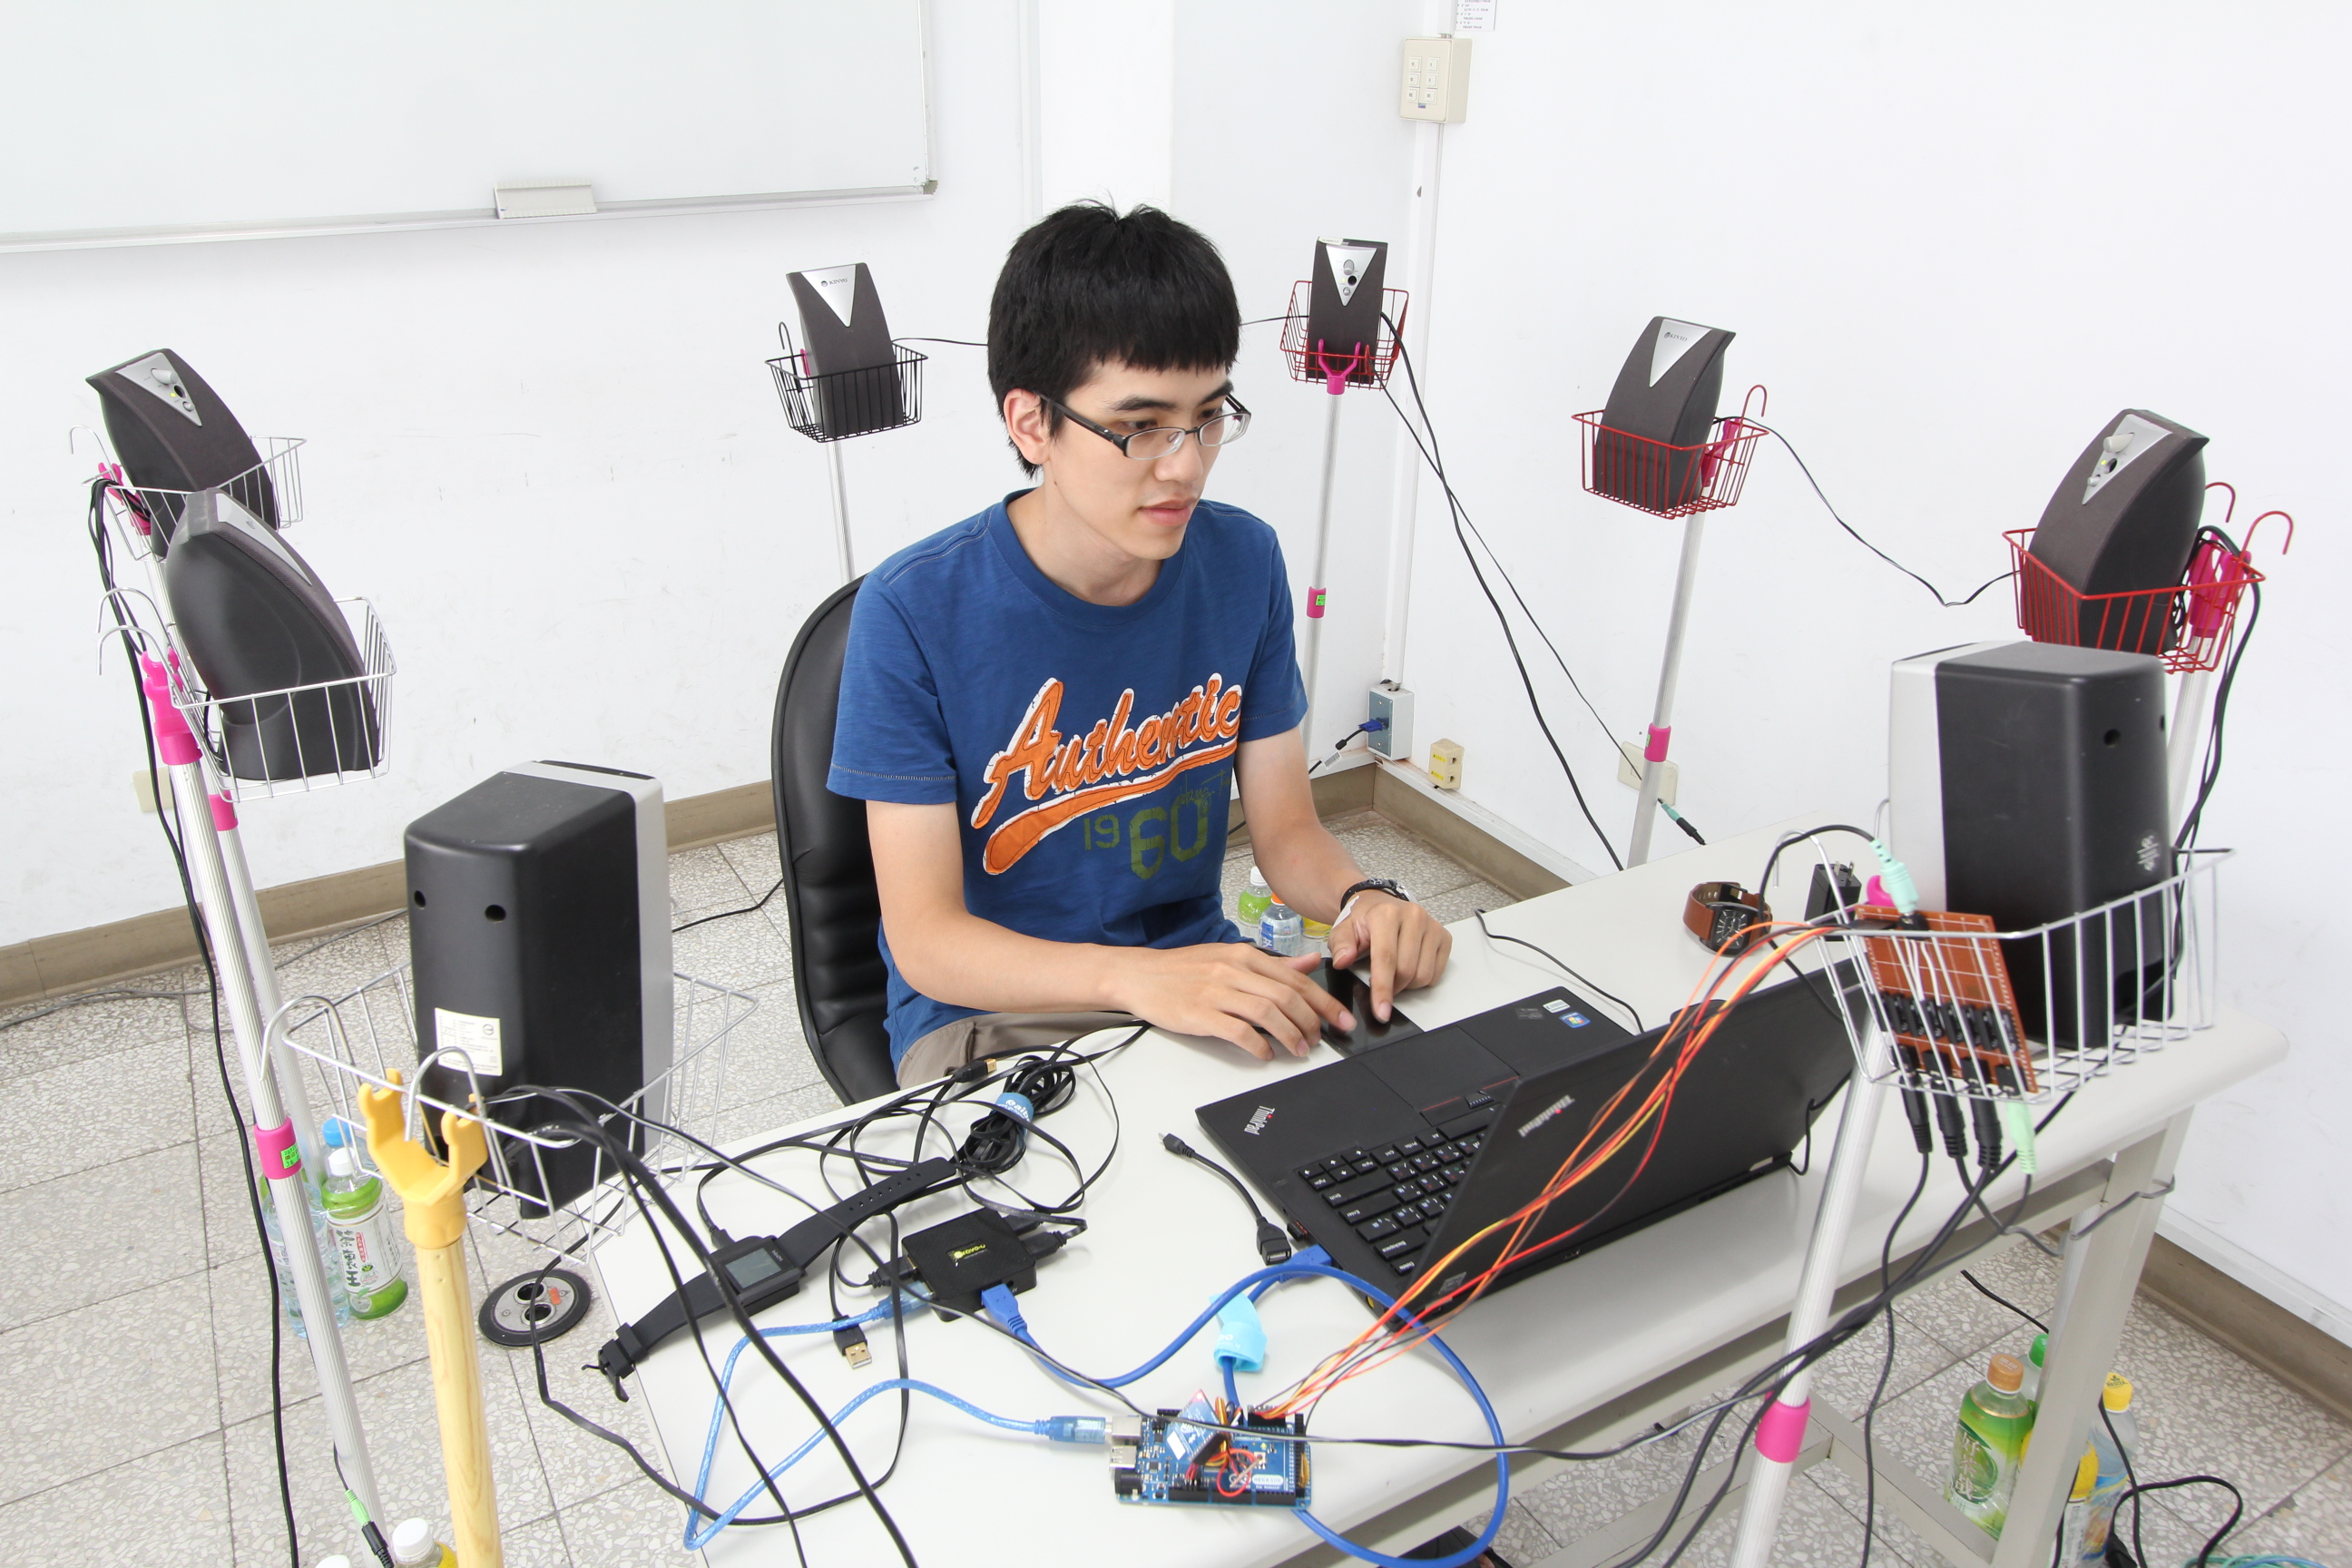
\includegraphics{Figure1}
%  \caption{Teaser Image}
%  \label{fig:teaser}
%}

\maketitle

\begin{abstract}
People with functional hearing use environmental sound as one of the sources to obtain information and learn what is happening in the surroundings. However, this type of media becomes less beneficial for people who are deaf or with hearing loss. This paper propose several wearable visual and tactile interfaces enable deaf and hearing-impaired people identify in which of the eight cardinal direction is the sound coming from. The study compared various types of encoding scheme being displayed on different accessories including a smartwatch, an eyeglasses, and a baseball cap for visual display devices. As well on the other hand, four vibro-tactile devices designed for three body locations were investigated: a hat, a belt, a wristband, and an armband. Prototype systems and applications were developed to evaluate performance and usability for each device and scheme through experimentations. Ten hearing-impaired subjects with different severity level participated in the experiment. The results showed an over all improvement in sound direction identification at over 60\% in accuracy and half the time less in response period when using visual and tactile assistive devices. Moreover, we reported on the users' preferences of accessories and display methods, and derived suggestions for the design of wearable assistive device.
\end{abstract}

\keywords{
	Visual display; vibro-tactile display; sound direction; deaf; hearing-impaired; wearable assistive device
}

\category{H.5.m.}{Information Interfaces and Presentation (e.g. HCI)}{Miscellaneous}

\section{Introduction}
Environmental sound is one of the sources that contain crucial information which allow human beings to learn what is happening in the surroundings. We are less likely to get hurt by something easily avoided if we heard it coming. However, this type of information becomes less beneficial for people who are deaf or hard-of-hearing. A simple interview were conducted with six hearing-impaired participants who use hearing aids (HIs) communicate and one of which uses cochlear implants (CIs). We found a common agreement from all participants that the existing hearing devices do not fully meet the needs of aiding them identify certain auditory information, namely the sound direction.

Congenitally, regular human beings use five traditional senses to perceive information from the living environment; they are sight, hearing, touch, smell, and taste. It is clear that most of the time humans rely on hearing to comprehend the location of the sound based on its time and intensity difference \cite{Wallach1939}. Despite that the remaining sensors cannot obtain acoustic information, it is however possible for human to perceive and recognize directions by using visual or tactile sensing stimuli. This can be seen from other studies that implement visual and tactile interface for various purposes including navigation and directional guidance of sound \cite{Borg,Kim2013,Tessendorf2011,Tsukada2004}.

Although previous studies demonstrated the feasibility of using these interfaces to assist localization of sound, but only few display methods and limited accessories were put to test. Moreover, some of the mentioned study did not carry out the experiments with hearing-impaired participants, and some did not undergo any user experience study. In this paper, we proposed a wider range of use on wearable devices with multiple types of visual and tactile cue display as a sensory aid to provide directional information of an environmental sound. The device aims to help people with hearing loss quickly identify the orientation of sound to create a better perception of the upcoming events. User experience and comprehensive performance evaluation between all designs were conducted.

We selected six body accessories for the design of seven assistive devices. They are baseball cap, eyeglasses, smartwatch, hat, wristband, and armband. The former three are used in visual display whereas the rest are implemented as vibro-tactile devices. It is noteworthy to mention this study is focused on evaluation of display methods and performance of such assistive devices. Hence, the sound detection was not considered within the design.

Since there has been numerous reports shown that people who are congenitally deaf have enhanced ability to capture more visual activity in the peripheral field than normal hearing individuals \cite{Bavelier2000,Dye2009, Codina2011a}, our design uses visual indicator in the periphery to inform hearing-impaired users the direction of a coming sound. The accessories chosen to perform visual information except smartwatch are worn close to the eyes and can be easily accessed via peripheral vision.

Information provided by tactile sense is relatively unobtrusive. It is suited for daily use in mobile environments. However, many existing devices such as cellular phones don't transmit complex information via the tactile sense due to the quantity and allocation of the vibration unit is limited by their design. Some research on navigation are able to use vibrators to performed directional information because the contact area of such tactile interface to human body is expended, and the quantity of vibration unit is multiplied. Ring shaped tactile interface appears most suitable to deliver notification that represent directions in a 360 $^\circ$ angle. The shape of a hat, belt, and wristband fit to such criteria. Since these accessories are wrapped around user's upper body, it gives the advantage to alleviate isolation of tactile sense from body motion produced by daily activity such as walking. In addition, the study designed an armband which the vibration units are formed in a 3 x 3 hollowed-square grid. We are interested to see if the scheme patterns can be distinguished by users and its performance compared to ring shaped devices.

Two experiments were conducted to compare performances and user experience on different devices applied with various encoding scheme. The goal of the previous experiment is to eliminate, based on performances, the types of encoding scheme that are inefficient and inaccurate. Moreover, the first experiment is split into two parts (1A and 1B) in order to analyze the usability and performances of visual and tactile displays individually. Twenty non-hearing-impaired people took part in the first experiment (ten for each part). In the second experiment, same procedure were carried out as the first but only the remaining display scheme are put to test. We asked ten hearing impaired participants to accomplish the tasks. Audio equipments are added in second experiment to simulate environmental sound in a real life setting.

The final result showed that visual and tactile assistive devices do help people with hearing-impairment better identify the sound source location. We compared results between participants wearing only HIs and CIs, and using our devices as assistant. Average user performance and accuracy had over 60\% improvement rate on all visual and tactile devices. The recognition time in average was also dropped by two seconds, almost half the time less than that with only His and CIs. Among all devices, visual display method appears to have better performance and user preferences. Nevertheless, smartwatch is the most prominent in many perspective. Even though the feasibility of real life application with these types of assistive device is still debatable, our results infer a great possibility and trend of implementation in future work. This requires further investigation.

\section{Related Work}
Research related to this study falls into two categories: tools for navigation, and tools for sound visualization. Regarding to the enhancement of acoustic awareness for deaf people, many research had proposed using visual feedback as wearable assistive interface. A glasses-type assistive device was designed to detect ambient sound from four directions by using various Microelectromechanical-systems (MEMS) microphones attached to the surface. Four LEDs are installed on the glasses to display directional estimation for deaf users \cite{Kim2013}. The prototype device in the study successfully displayed the estimated direction to user via visual display. However, instead of investigating usability and preferences via visual interface, the research was mainly focused on the algorithm used for estimating direction. Hence, there were no experimentation conducted with real participants nor discussion related to its design. A British artist and designer elaborated a project to design a pair of shoes that is capable to navigate its owner to any destination using build-in GPS and light indicator on the shoes \cite{Wilcox2012}. Although the interface design sufficiently displayed directional information to user, but due to the fact that the shoes are normally not within sight, it is unable to provide immediate notification when necessary.

Another approach using augmented reality system to assist hearing impaired visualize sound source location in indoor settings were proposed in \cite{Shen2012}. The system recognized the sound source and its location using acoustic processing. Then it notifies the user through different visual markers by augmented visioning. In addition, several other research investigate types of forms of visual display and display devices for providing awareness of environmental audio to deaf individuals. The studies include evaluations of various figure representation such as iconic imagery, spectrograph, and ripples, that will be exhibited on large displays, for instance, personal computers, televisions, and even ceiling \cite{Ho-Ching2003,Matthews2006a,Matthews2005,Tomitsch2007}. All the previous works mentioned seems to be promising to deliver useful information. They are, however, lacking the characteristic of mobility and feasibility in outdoor settings.

Many studies on human navigation systems and location-aware information services proposed various forms of wearable interfaces such as glasses, gloves, shoes, vests, and so on. Research in regards with wearable tactile interfaces has been carried out, such as Cyber Touch \cite{CyberGlove}, GentleGuide \cite{Bosman2003}, a tactile display vest by Tan et al. \cite{Tan1997}, and ActiveBelt \cite{Tsukada2004}. Cyber Touch can generate tactile feedbacks of objects in virtual world, using six vibrators attached on gloves. GentleGuide proposed a tactile navigation system via two bracelets. It outputs three commands, left, right, and stop. A pair of glasses enhanced with 4 vibrators and 3 microphones with the purpose to locate sound sources for visually and hearing impaired people was presented in \cite{Borg}. In the meanwhile, we conduct an investigation with our approach using eight vibrators and various display patterns, which we believed users can obtain directional information more intuitively.
 
Two popular forms of wearable tactile interface are designed on vests and belts. Several applications of simulating directional lines and geometric patterns on tactile display are proposed in \cite{Tan1997}. They attached a matrix of vibrators to the back of a vest, and tried transmitting directions and other information to user. Another research on tactile displays implemented a similar technique in aircraft cockpits \cite{Raj2000}. The project used a vest-type tactile displays to provide pilots with navigational information. In our study, we tried scaling down the vest model to a size of an armband so fits on the forearm. ActiveBelt is an example of a belt-type tactile display. It is a waist belt with GPS sensor and eight vibration motors installed that enables users to obtain multiple directional information for navigation purposes.

In conclusion, many related works had been done previously to report the usability and performances of visual and tactile devices. However, most of them are aimed to provide directional information solely for navigation purposes. Others proposed application for helping the deaf improve their acoustic awareness with certain types of device, but they are only applicable on certain parts of the body location. There are no comprehensive comparison and evaluation between all the possible interfaces and display methods of sound source localization for people with hearing loss.

\begin{figure*}[!t]
\centering
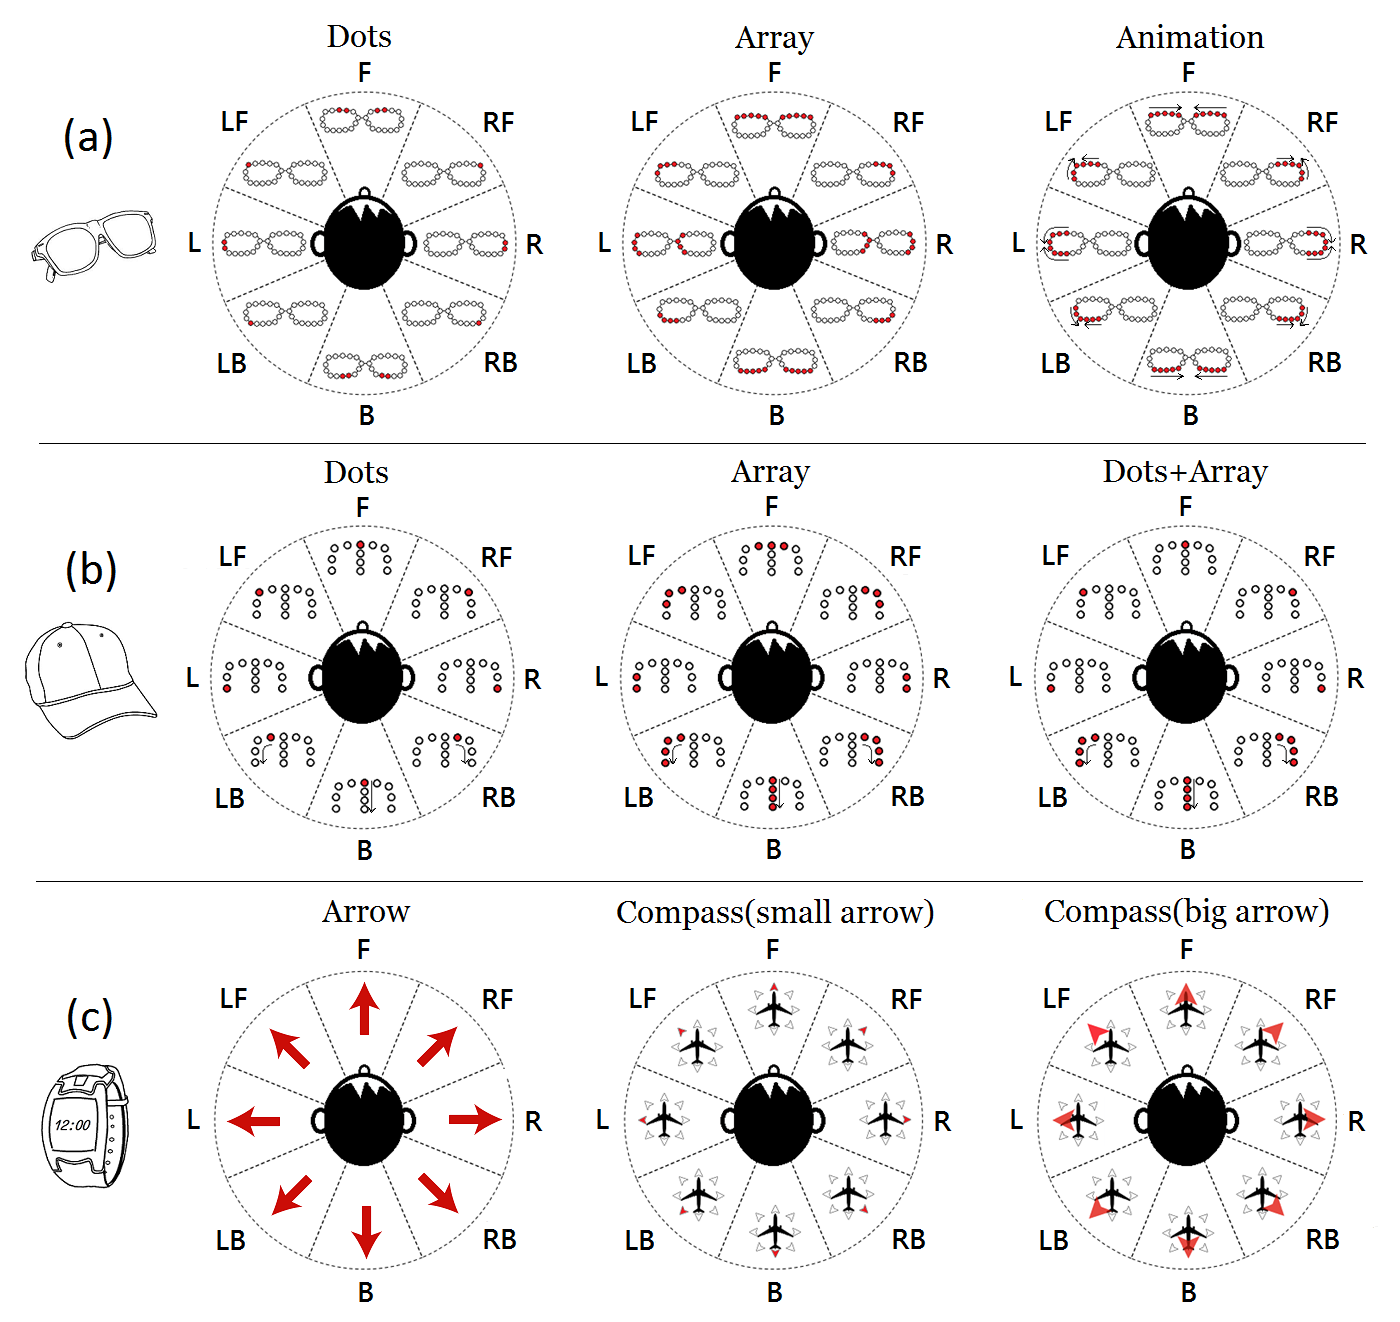
\includegraphics[width=2.15\columnwidth]{visual_pattern_combine}
\caption{LED glasses pattern schemes.}
\label{fig:all_scheme}
\end{figure*}

%\begin{figure*}[!t]
%\centering
%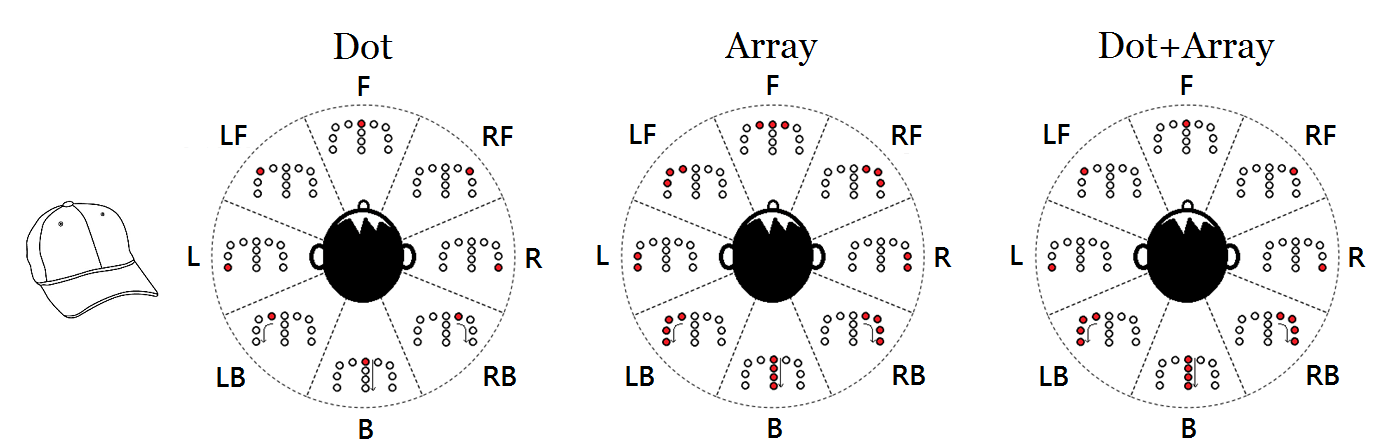
\includegraphics[width=2.15\columnwidth]{hat_pattern_combine}
%\caption{LED cap pattern schemes.}
%\label{fig:cap_scheme}
%\end{figure*}
%
%\begin{figure*}[!t]
%\centering
%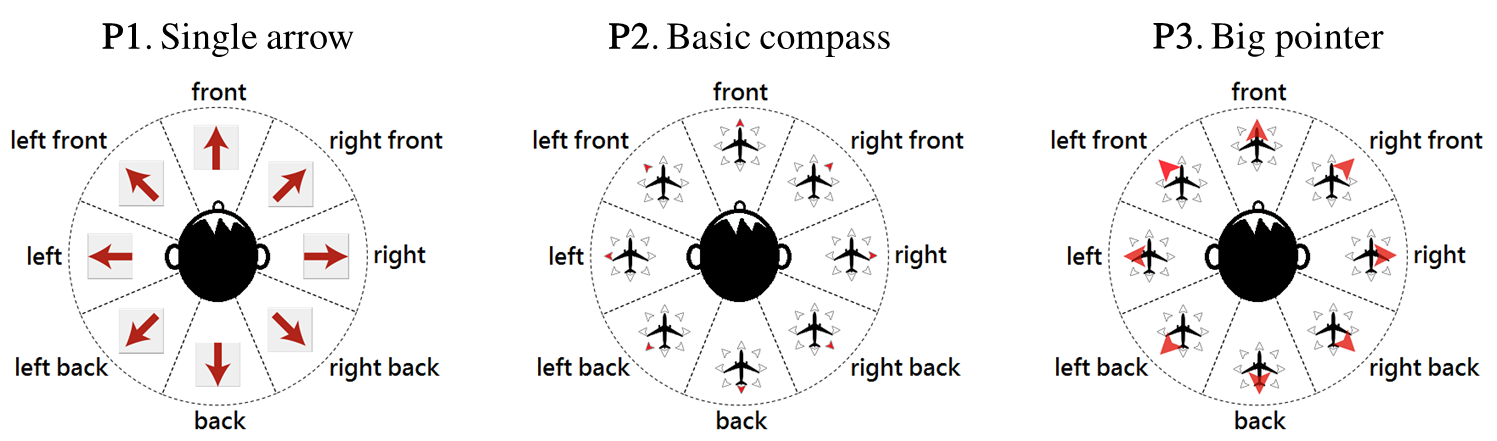
\includegraphics[width=2.15\columnwidth]{smartwatch_pattern_combine}
%\caption{Smartwatch pattern schemes.}
%\label{fig:smartwatch_scheme}
%\end{figure*}
%
\begin{figure*}[!t]
\centering
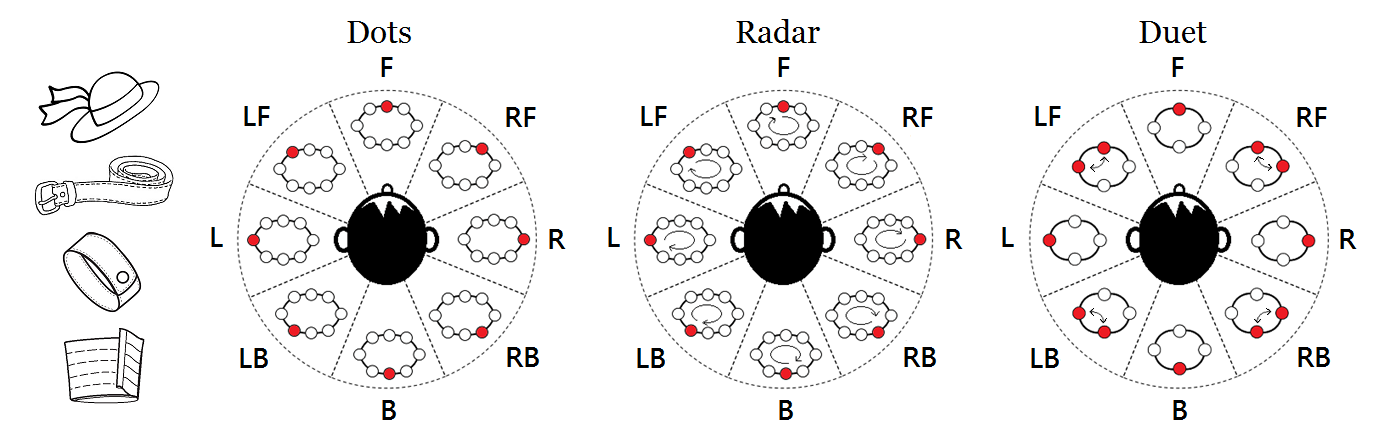
\includegraphics[width=2.15\columnwidth]{vibration_pattern_combine2}
\caption{Vibration devices pattern schemes.}
\label{fig:vibratin_scheme}
\end{figure*}

%\section{Choosing of Wearable Visual Accessories}
%There has been numerous reports shown that congenitally deaf and hard-of-hearing people have enhanced ability to capture more visual activity in the peripheral visual field than normal hearing individuals \cite{Bavelier2000,Dye2009}. In previous studies, experimentation were carried out to compare deaf and hearing group in performance of both their peripheral and central visual attention; participants are asked to click a button in response when a periphery or central stimuli is presented. The deaf individuals exhibit enhanced performance, in terms of faster reaction time and higher accuracy rate, for tasks performed in the visual periphery. And this effect is even more evident when subjects are adolescents \cite{Codina2011a,Codina2011}.

%Granted that deaf and hard-of-hearing people can see better in peripheral vision space, therefore we propose using visual indicator in the periphery to inform them the direction of a coming sound. Hence, several body accessories are chosen to implement in our study, which includes a smartwatch, a pair of glasses, and a baseball cap. These accessories share a common characteristic which is near the vision field while applied or can be easily engaged with our eyes when feedbacks are performed.

%\section{Choosing of Wearable Tactile Accessories}
%Since the information provided by tactile sense is relatively unobtrusive, it is suited for daily use in mobile environments. However, many existing devices don't transmit complex information via the tactile sense due to the quantity and allocation of the vibration unit is limited by their design. Most of them send only simple signals, such as vibration in cellular phones. Some research on navigation are able to use vibrators to performed directional information, because the contact area of the tactile interface to human body are expended, and the quantity of vibration unit are multiplied.

%We have focused on three type of accessories: hat, belt, and watch. The shape of these devices seems suitable to transmit directional information via the tactile sense. Since these accessories are wrapped around user's body when being worn, it is possible to provide directional information by applying vibration stimuli from any angle at such body part. User can perceive vibration clearly even in moving. Moreover, since many people usually wear hats, belts, or watches they don't need to wear additional devices. In addition to the accessories mentioned above, we designed an armband which we are interested to see if user can distinguish the directional patterns performed by a square-shaped vibration array that will be strapped on the back of user's forearm. Eight vibrators are well-distributed and stitched inside each device.

\section{Prototype and Pattern Design}

Each prototype devices is designed to convey signals in eight directions corresponding to user's position. This was proposed in \cite{Tessendorf2011} to minimizes the perceptual error. A set of visual and vibro-tactile encoding schemes suitable for directional pointing of target angles in the complete 360$^\circ$-range are mapped out and shown in figure \ref{fig:all_scheme}.

\subsection{Visual Devices}
Three types of accessories are used to implement in visual display: glasses, baseball cap, and smartwatch. Due to the shape and size of each device are noticeably different, we designed three types of encoded schemes for each accessory. Except for smartwatch, which uses its native display panel and runs micro App to display sign imagery, glasses and baseball cap are both equipped with multiple yellow-greenish LEDs to indicate directions of sound source. The display patterns for cap and glasses share common design concept but differ in the arrangement of LEDs. 

%\begin{figure}[!b]
%\centering
%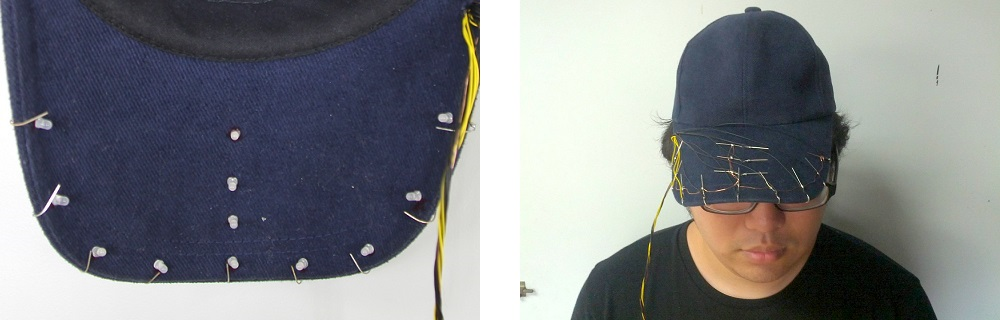
\includegraphics[width=0.9\columnwidth]{cap_4}
%\caption{LED cap.}
%\label{fig:cap}
%\end{figure}
%
%\begin{figure}[!b]
%\centering
%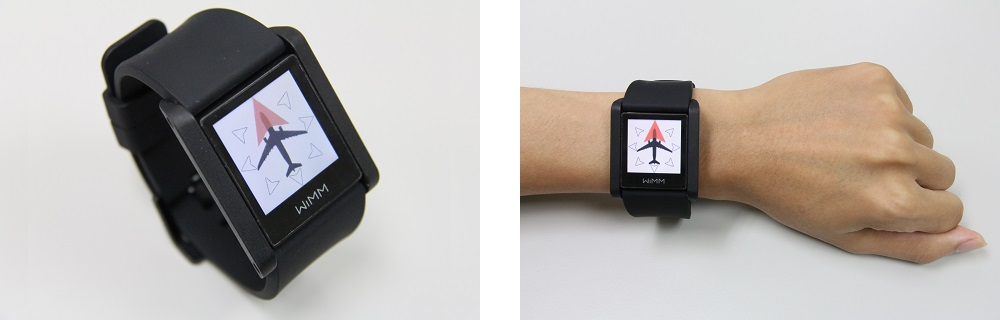
\includegraphics[width=0.9\columnwidth]{smartwatch_4}
%\caption{Smartwatch.}
%\label{fig:watch}
%\end{figure}

%\begin{table}
%\centering
%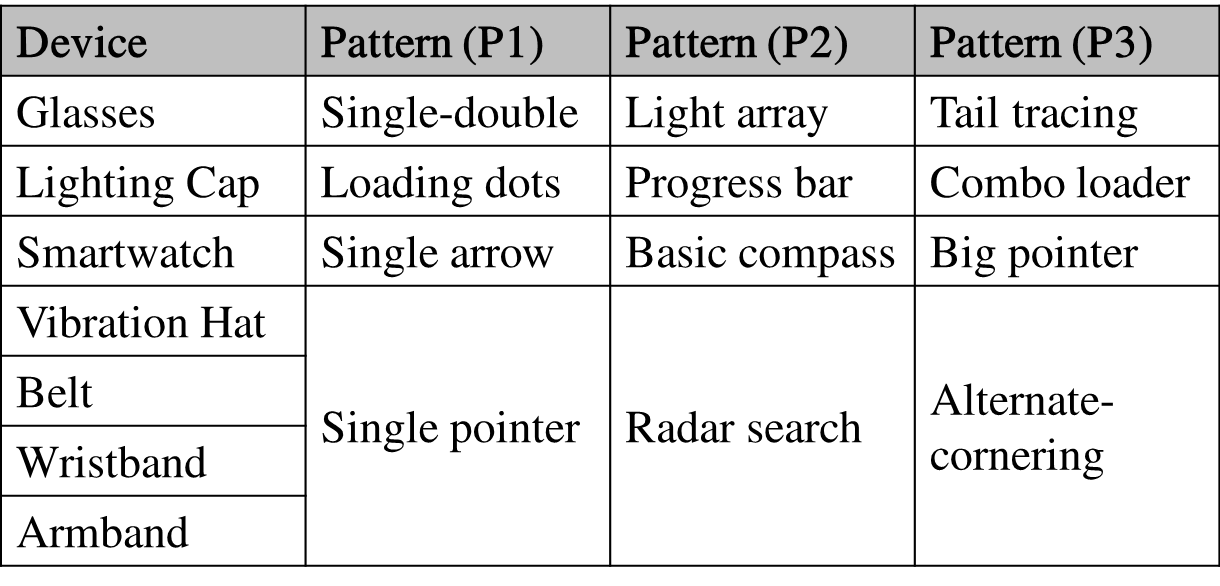
\includegraphics[width=\columnwidth]{pattern_chart}
%\caption{A list of devices and names of each designed pattern.}
%\label{tab:pattern_chart}
%\end{table}

\subsubsection{Glasses}
To perform complex display patterns, a high density LEDs setup is installed around the glasses frame. We use a regular lensless glasses as the base of the prototype. Small holes were drilled around its frame in order to install LEDs. Electrical wires are connected to the LEDs and strapped around the frame rims and bundled alongside the temples (see Figure~\ref{fig:visual_devices}a). There are 28 LEDs in total (14 on each side of the glasses), and they are evenly distributed across the frame rims in a circular formation. The tip of LEDs are bent inward to point at the user's eyes so the light can be seen easily while emitting.

Three patterns are designed to used on glasses, which are: \textquotedblleft Dots\textquotedblright, \textquotedblleft Array\textquotedblright, and \textquotedblleft Animation\textquotedblright. In the first two patterns, all configured LEDs blink together continuously, whereas in the third configuration the LEDs are turned on in a gradual motion and turned off the same way recursively, similar to an electronic marquee.

In the \textquotedblleft Dots\textquotedblright  setting, the glasses indicates four relative directions (front, back, left, and right) using two or a pair of two LEDs which blink simultaneously; and only one will blink at the corner when indicating diagonal directions. In the second pattern, \textquotedblleft  Array\textquotedblright, a whole set of LEDs are lit up together on each side of the rim representing the respective direction. Diagonal directions are performed by lighting up multiple LEDs on each corner. The last pattern is more complex; front and back are displayed in sliding motion, which will appear to user as two beams of lights running through the rim entering from each side of the glasses and disappearing in the middle. Whilst left and right are presented with lights running from mid-top and mid-bottom rims toward the according side, then disappear at the point where both light beams meet on the side of the glasses. For diagonal direction, both side of the adjacent rims of the corresponding corner lights up in gradual motion toward the corner itself then disappear in same order as appearance.

Since the surface of the glasses is flat and vertical, our designed pattern are then displayed in a vertical format. Therefore, it is necessary for user to remap the given directional information from vertical to horizontal space. For instance, if LEDs are blinking on the top rim of the glasses, it means that the sound is coming from the front relative to user. On the other hand, if LEDs blink on the bottom side of the glasses, it indicates the sound is coming from behind. It is considered that some user may think reversely (i.e., top as back, and bottom as front) due to intuition or by custom. We put this aspect in observation with the experiment by asking users whether they felt the need to reverse the setting.

\begin{figure}[!b]
\centering
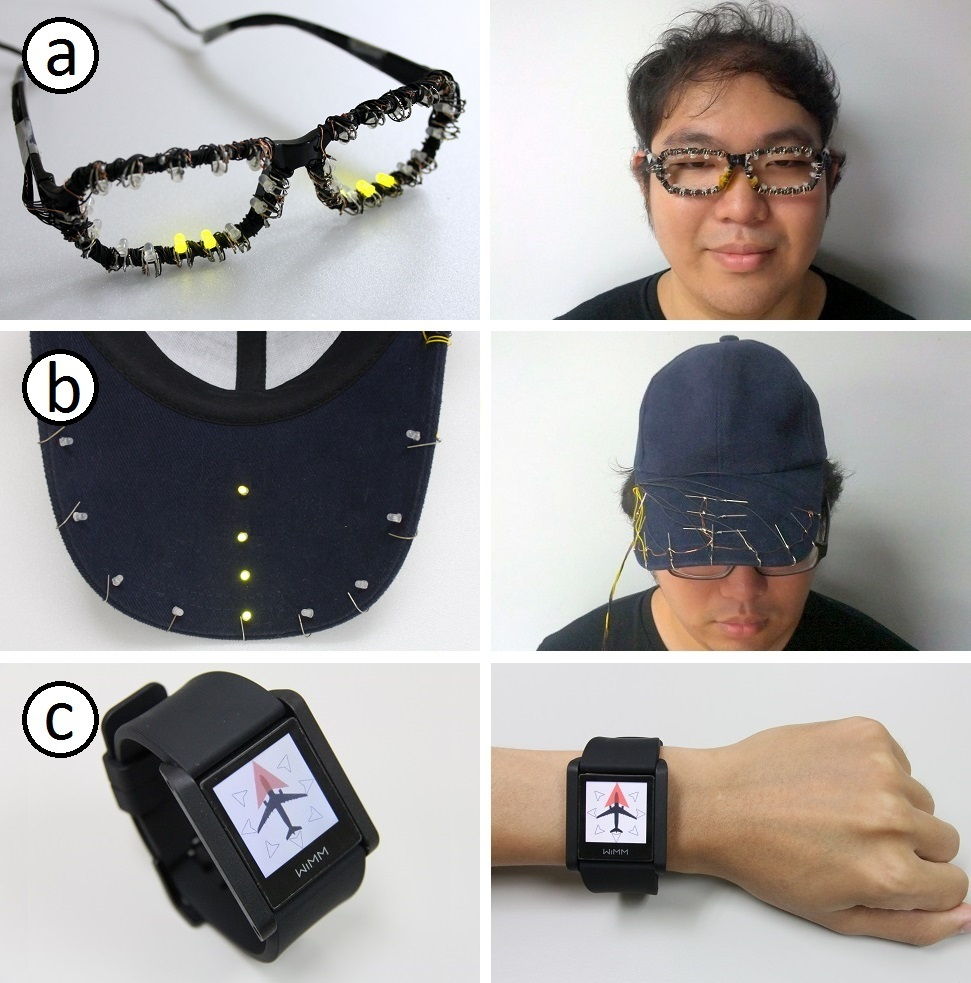
\includegraphics[width=\columnwidth]{prototype_visual3}
\caption{LED devices.}
\label{fig:visual_devices}
\end{figure}


\subsubsection{Cap}
A normal-sized baseball cap is used for the study. It has bill of approximately 17.78 cm (7 in.) x 9.5 cm (3.74 in.) in dimension. LEDs are installed on the bill of the cap in the shape of a trident tip (see Figure~\ref{fig:visual_devices}b). The LEDs are pinned through the bill and facing down toward the user. Wires are connected to the LEDs on top of the bill and bundled on the right corner of the bill.

Different than the glasses, we are able to design a set of horizontal display patterns since the bill is close to a flat surface. Nonetheless, when it is worn, the area of which human eyes can see using peripheral vision is limited. We propose three display patterns which are \textquotedblleft Dots\textquotedblright, \textquotedblleft Array\textquotedblright, and \textquotedblleft Dots+Array\textquotedblright.

Three types of display patterns are designed base on the arrangement of the trident-shaped LEDs setup. \textquotedblleft Dots\textquotedblright pattern performs orientational information using only one LED for all directions in the field of view (FOV), i.e. front, left, right, front-left, and front-right. The remaining three directions on the back are displayed by using single LED which jumps backward toward the user's head. The second method, \textquotedblleft Array\textquotedblright, turns on two or more lights to present directions in the FOV. For the backward directions, it is displayed with an array of LEDs lit backward progressively. The last pattern is a combination of previous two; it is composed of single blinking LED for FOV angles and the display patterns of \textquotedblleft Array\textquotedblright for backward directions.

\subsubsection{Smartwatch}
We use \textit{WIMM One} smartwatch manufactured by \textit{WIMM Labs} for wrist-worn prototype (see Figure~\ref{fig:visual_devices}c). The smartwatch runs on a modified Android platform of version 2.1, and it is equipped with a 160 x 160 pixel, 2.5 cm (1.0 in.) square display. For this study, we created a micro App to display images to represent directional information. The difference between smartwatch and other devices is that it uses native display panel to show directions rather than using LEDs. Plus, it uses the build-in vibration feature as part of the notification alert.

Using different designs of imagery, we proposed three types of representation of directions. They are \textquotedblleft Arrow\textquotedblright, \textquotedblleft Compass (small arrow)\textquotedblright, and \textquotedblleft Compass (big arrow)\textquotedblright. The first type displays large arrows to indicate directions, and each arrow occupies the whole display which allow user to see clearly. The second design implements similar concept as a compass; with eight arrows pointing at eight cardinal directions on the panel, one of which is colored in red at a time   to indicate direction. An image of an airplane is put in the middle to show the relative orientation to the colored arrow. The third type is fairly identical to the second except the size of the colored arrow is significantly larger than the rest when directions are displayed.

\subsection{Tactile Devices}
Four accessories are designed to perform experiment: hat, belt, wristband, and armband. Eight vibrators are well-distributed and stitched inside each device. We evaluated a wide range of vibrators and selected coin-shaped vibrators with a diameter of 10 mm (310-103 Vibration Motor 2.7 mm Button Type from Precision Microdrives) that have been developed for vibro-tactile feedback in hand-held applications. In order to clearly distinguish each individual vibrator and prevent misinterpretation, isolating shock waves between each vibrators is fairly important. Since the shape and vibrator arrangement of all tactile devices are similar, all of the designed patterns for tactual sense are suitable for every device. 


%\begin{figure}[!b]
%\centering
%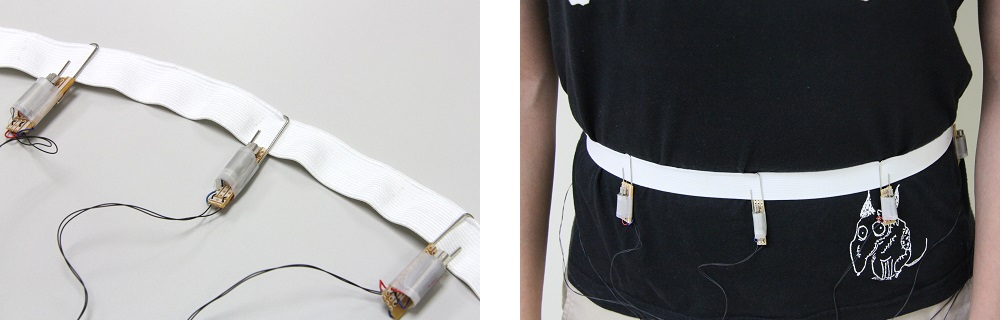
\includegraphics[width=0.9\columnwidth]{belt_4}
%\caption{Belt.}
%\label{fig:belt}
%\end{figure}
%
%\begin{figure}[!b]
%\centering
%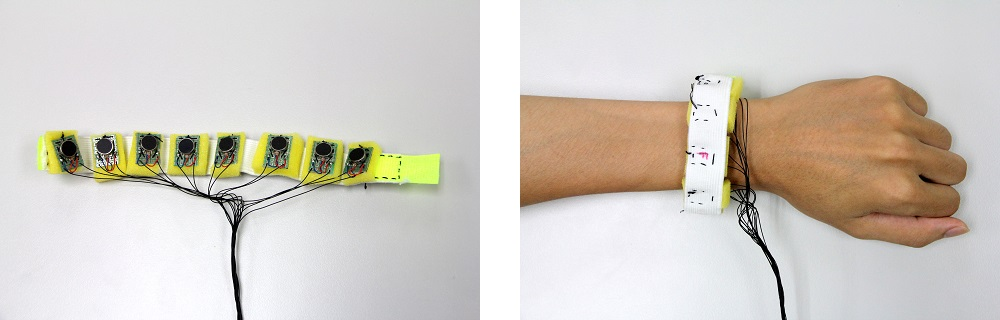
\includegraphics[width=0.9\columnwidth]{wristband_4}
%\caption{Wristband.}
%\label{fig:wristband}
%\end{figure}
%
%\begin{figure}[!b]
%\centering
%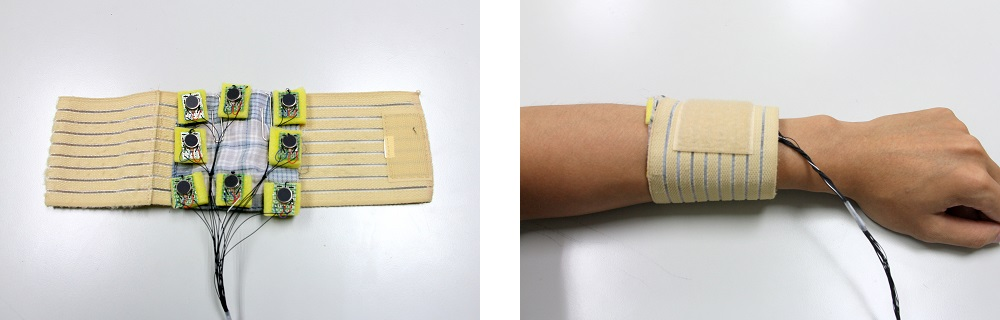
\includegraphics[width=0.9\columnwidth]{armband_4}
%\caption{Armband.}
%\label{fig:armband}
%\end{figure}

\subsubsection{Hat}
The hat is compose of soft material which aimed to avoid unwanted propagation of vibration sense through conduction. Eight vibrators are distributed evenly around the hat (see Figure~\ref{fig:vibration_devices}a).

\subsubsection{Belt}
Since every user's waistline is predictively different. We designed a universal-size belt that consists of adjustable clips in which the vibrators are attached and elastic strip fit to majority of the users (see Figure~\ref{fig:vibration_devices}b). Moreover, to ensure the output is strong enough to be sensed through clothings, we use cylindrical-shaped vibrators with diameter of 5 mm, length of 20 mm to perform stronger vibration.

\subsubsection{Wristband}
The watch function is unconcerned in the study of tactile design. Therefore, we emulate the integration of vibro-tactile interface into a watch band by enhancing a wristband with vibrators which are arranged circularly around user's wrist (see Figure~\ref{fig:vibration_devices}c). We have wired each vibrators loosely on an elastic band and every vibrator is fixed on a foam-rubber cushion to isolate the shock wave from each other.

\subsubsection{Armband}
Different from the previous accessories, this device is made up of a square-shaped vibration array that will be strapped onto the back of user's forearm using a semi-elastic sport bandage (see Figure~\ref{fig:vibration_devices}d). As the design of the wristband, each vibrator is positioned on an isolated foam-rubber to prevent unnecessary conduction. The size of vibration array is 10 cm x 10 cm.

\begin{figure}[!t]
\centering
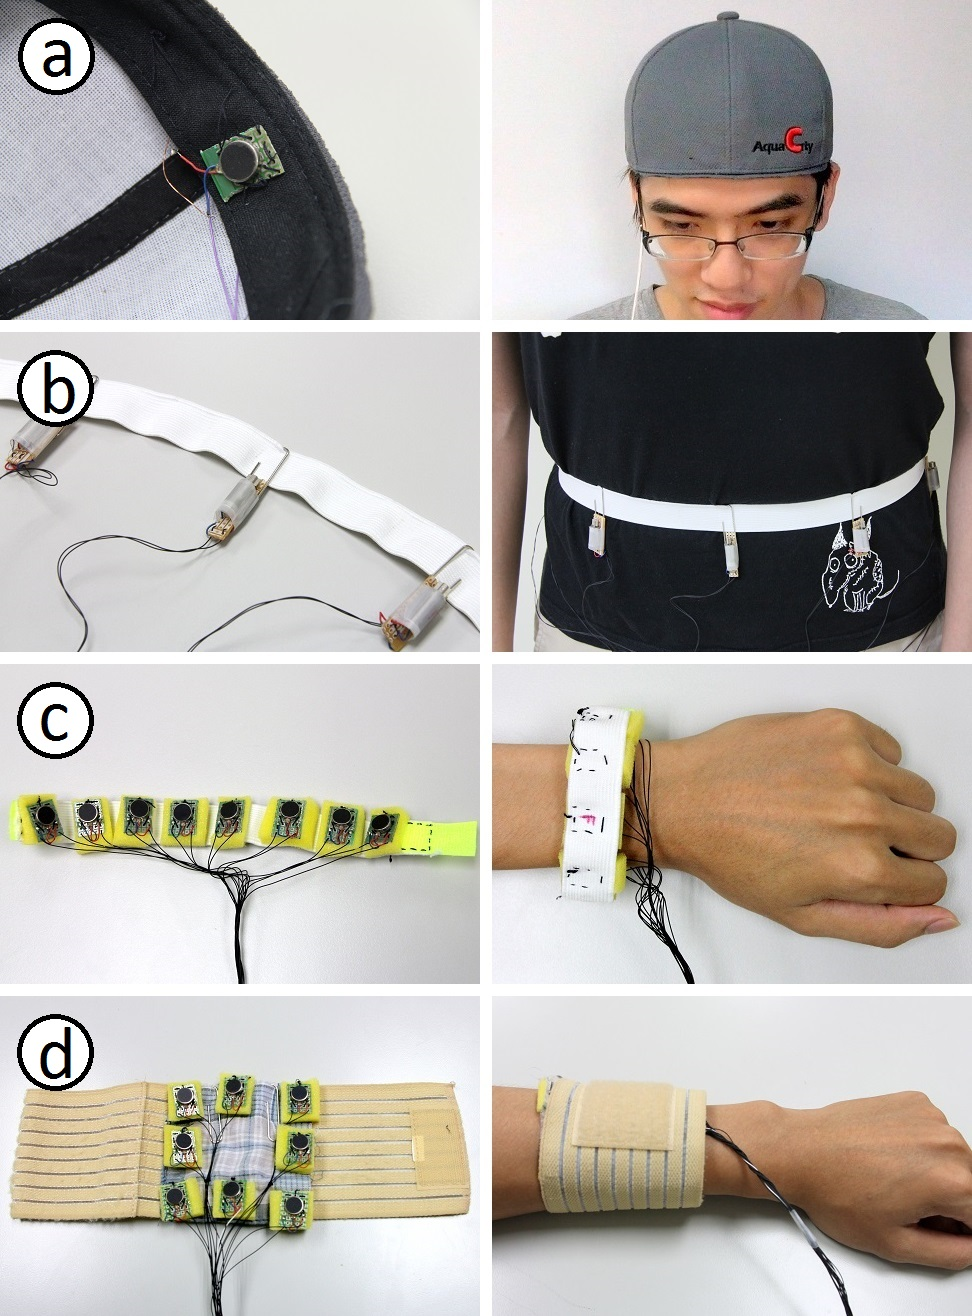
\includegraphics[width=\columnwidth]{prototype_vibro2}
\caption{Vibration devices.}
\label{fig:vibration_devices}
\end{figure}

\subsubsection{Patterns for Tactile Device}
Thinking of possible patterns that can provide directional information by vibrators, we designed three distinguish patterns: \textquotedblleft Dots\textquotedblright, \textquotedblleft Radar\textquotedblright, and \textquotedblleft Duet\textquotedblright.
All of the patterns are running in a continuous on-off fashion.

The first pattern is performed by single vibrator activated at a time to represent individual direction. In the second display pattern, all vibrators are turned on one after another in clockwise order starting from the pointing direction with a longer pulse of vibration. 

The third pattern is operated using four vibrators; four absolute directions: front, back, left, and right are performed by single vibrator allocated on relative location like the first pattern, and the corner directions is represented by nearby two vibrators activating alternately. For example, front-right is indicated by vibrating front and right unit alternately.

Each of the designed patterns are proposed to withhold certain advantage. Discard the first basic pattern for instance, we hypothesis the alternate-cornering can reduce the difficulty of distinguishing the vibrator in high density array settings; radar search can help user easily recognize relative position of each vibrator in the array; and the singular radar will present the one direction in fixed position continuously therefore easier to grasp.

\section{Experiment 1}
\subsection{Experiment Description}
Our primary interest in experiment 1 is to understand which devices and which patterns are intuitively chosen by the users. The experiment requires participants to wear each of our devices alternatively and perform the experimental tasks. In each task, participants are asked to interpret directional information that our device delivered. At the end of the experiment, we filtered out the inefficient patterns and devices by analyzing the error rate and response time of each participant which are recorded during experiment. The first experiment is separated into two parts (experiment 1A and 1B) for the purpose of alleviating task loads per experiment. Therefore we will conduct the study and evaluation of visual and tactile devices separately.

\subsection{Apparatus}
The experiment was conducted using a mobile device (\textit{Galaxy Nexus}, running Android platform ver. 4.2.2), an Arduino Mega 2560 R3 (a bluetooth module, \textit{Bluetooth Bee} is added to the board), and the proposed wearable devices. The wearable devices are connected to Arduino. They can be remotely controlled via bluetooth using a mobile application we created for the exchange of task commands between hardware and recording user's answer during experiment.

\subsection{Participants}
Since the purpose of the experiment at this stage is to pick out the most efficient and intuitive devices and patterns, user’s hearing ability is not directly relevant to the outcome. Therefore, we found 20 hearing individuals (8 males, average 22.6) volunteered to participate in the first study. The participants are in a variety of academic backgrounds, such as advertising, management, ocean engineering, computer engineering and etc. Regardless of age, we distribute the number of participants evenly in terms of gender to take part in each of the experiment (1A and 1B).

\subsection{Procedure}

%\begin{figure}[!t]
%\centering
%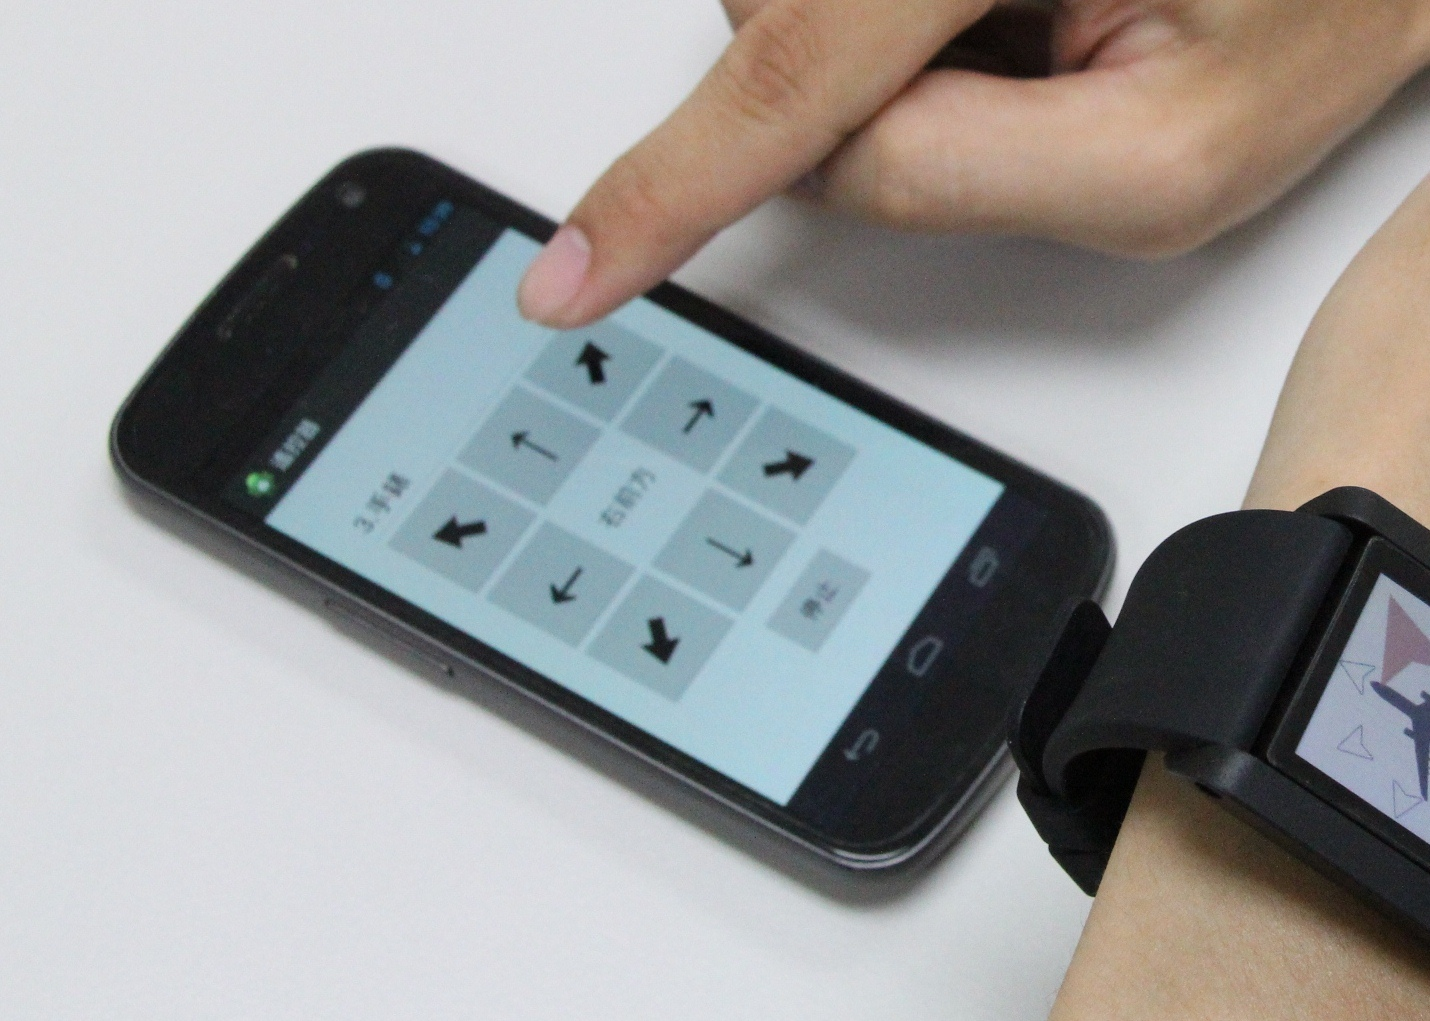
\includegraphics[width=0.9\columnwidth]{MobilePhone2}
%\caption{Mobile application for answer selection.}
%\label{fig:mobilephone}
%\end{figure}

The experiment for tactile devices consist of 12 tests (3 cue types x 4 devices), and 9 tests (3 cue types x 3 devices) for visual devices. The tests are sub-divided into sets of 3 (3 patters per device). Each test include 16 trials of tasks (2 repeated tasks for each of the eight cardinal directions given in random order). At the beginning of each test, we briefly explained and demonstrated the device and its pattern. Participants are given 90 seconds to learn each pattern on their own in practice mode. During the test when each pattern are presented, participants were instructed to choose an answer from the mobile screen as fast and accurate as possible. 10 seconds were given for each trial to make selection otherwise the system automatically skips to next question. The order of the devices and patterns in each part of the experiment was counterbalanced. The system records the response time and selected answer of each device and pattern. At the end of each test set, participants were asked to fill in a short questionnaire providing comments and ratings for each of the pattern using a Likert scale. Lastly, after all tests were finished, participants were asked to give ratings for each device. Any further comments or feedbacks are also recorded in the questionnaire.

\begin{figure}[!t]
\centering
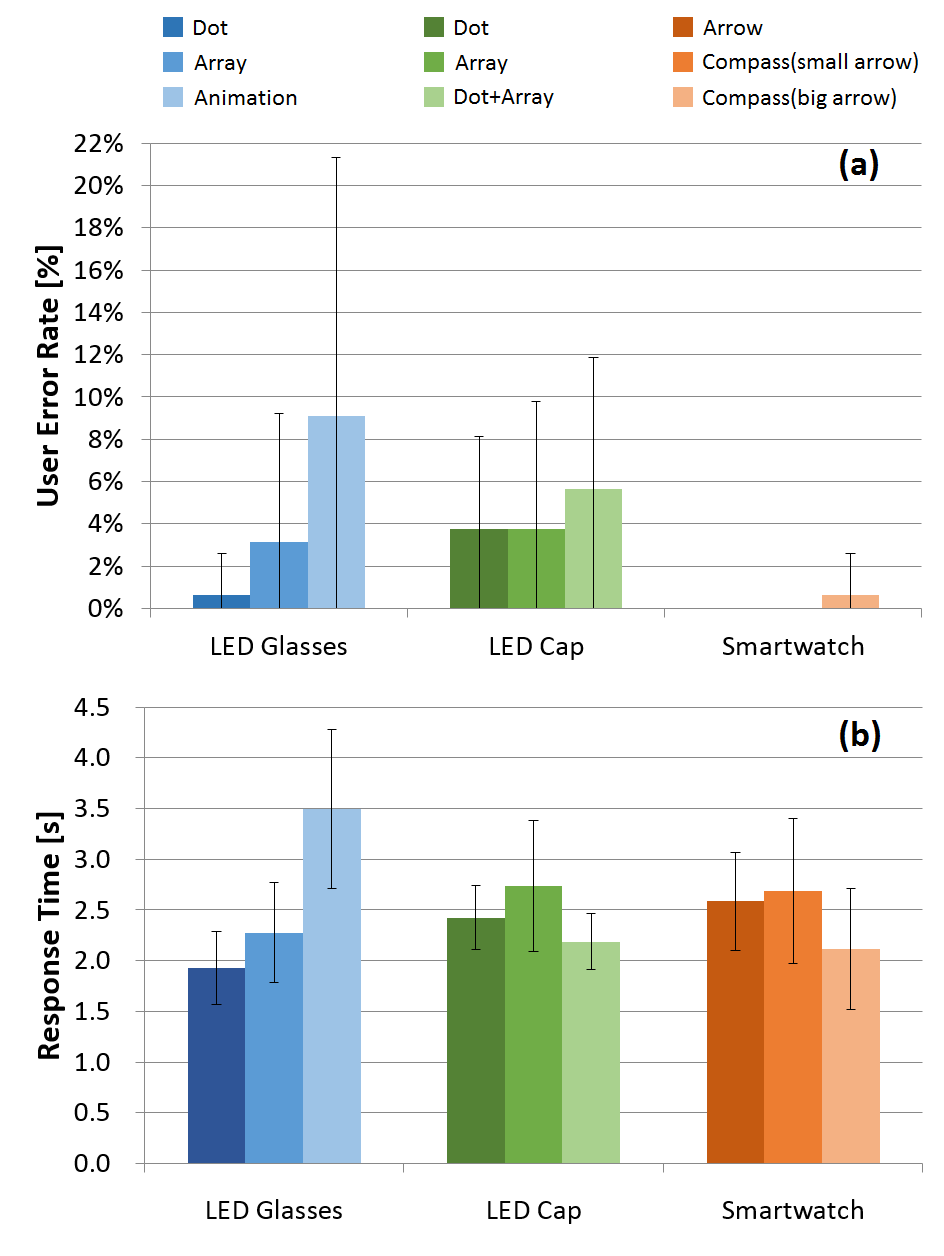
\includegraphics[width=\columnwidth]{stage1_Visual_ER&RT}
\caption{Mean error rate: Visual devices.}
\label{fig:visual_ER&RT}
\end{figure}

%\begin{figure}[!t]
%\centering
%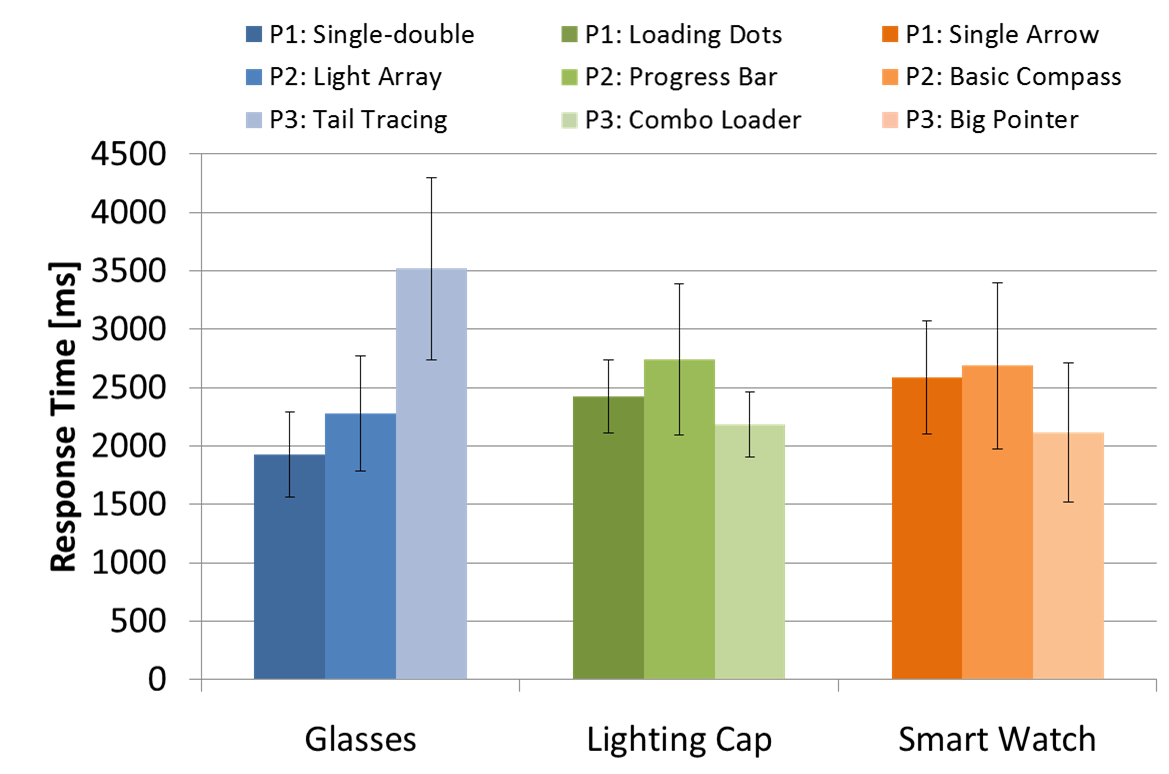
\includegraphics[width=\columnwidth]{Visual_RT}
%\caption{Mean response time: Visual devices.}
%\label{fig:Visual_RT}
%\end{figure}

\subsection{Experiment 1A Result: Visual Display}
Unlike tactile devices, the patterns designed between each wearable visual device are irrelevant to each other. Hence the result for each device is discussed separately. Figure~\ref{fig:visual_ER&RT} summarize the detection results of Experiment 1A. Both first and second pattern of smartwatch has gotten 0\% error rate. Although the third pattern has an error rate of 0.63\% higher than others, it is still considerably low. Surprisingly, the response time for third pattern of smartwatch is the shortest (2114 ms); about half a second faster than the others. This difference is confirmed by repeated-measured ANOVA (RMANOVA), F(2.8)=11.563, P\textless0.05. Few participants stated that the distinctive size of the indication arrow makes it easier to identify. And overall, smartwatch has the lowest error rate among all devices whereas in contrast, LED cap obtained the highest.

The error rate of pattern three for glasses is noticeably higher than the others (9.09\%), but the first pattern is only 0.63\%. However, RMANOVA results show no significant difference in between the three. In terms of detection time, there was a statistically significant difference, F(2,8)=24.470, p\textless0.05. The response time for pattern three exceeded the first by almost 1500 ms. This result match with the statement from two of the participants: \textquotedblleft First pattern of the glasses is sufficient and clear, and the animation used in the third pattern is time consuming and sometimes confusing.\textquotedblright

Error rates of the first and second pattern for cap are the same, both at a rate of 3.75\%. Even though the third is a bit higher (5.63\%) than the rest, the response time for third pattern is however the shortest among the three at 2187 ms. RMANOVA shows a significant difference of response time (F(2,8)=7.006, P\textless0.05) among the three but not error rate. Most participants said the first single blinking pattern is enough and better than the second, and few of them mentioned that the difference between the two methods showing backward directions are unnoticeable. Overall, by the scale of preferences, cap is voted the most preferred whereas glasses are the least. Although error rate of the glasses is a bit lower than cap, half of the participants reported that the blinking LEDs in front of their eyes makes them uncomfortable.

\subsection{Experiment 1A Conclusion}
The performance of the smartwatch is relatively high in terms of high accuracy. Since the smartwatch use simple imagery to display directional information, it is fairly easy for users to understand at a glance. We also discovered that when using relative positioning and referential sizing of icons to present directional information will raise the efficiency and intuitiveness for users to determine.

The glasses have the lowest error rate in one of the patterns which use two or less LEDs and simple blinking to represent directions. As the amount of LED lights increase, the performance and comfort level decreases dramatically. It is caused by two reasons: 1) one is that the brightness level is too high therefore brings burden to the eyes, and another is that 2) the surface of the glasses is too small to display complex patterns, it causes confusion when information are crammed together or overlaps each other. However, if appropriate lighting and position is considered when displaying information near the eyes, the outcome can be efficient. Due to the fact that when information is displayed, the interface can directly and immediately interact with the user's eyes on sight. Users are then unlikely to miss important notification. Also, this process would not require too much physical activity to access the intended information, such as moving the head or raising the arm.

Lastly, the preference of the patterns on the cap shows a common principal as the glasses, \textquotedblleft the simpler the better\textquotedblright. Users tend to prefer single blinking LED than complex and overlapping. In conclusion, for this experiment we have selected three patterns, big-arrow compass, single-double, and light jumper, one from each device to continue with the second experimentation.

\begin{figure}[!t]
\centering
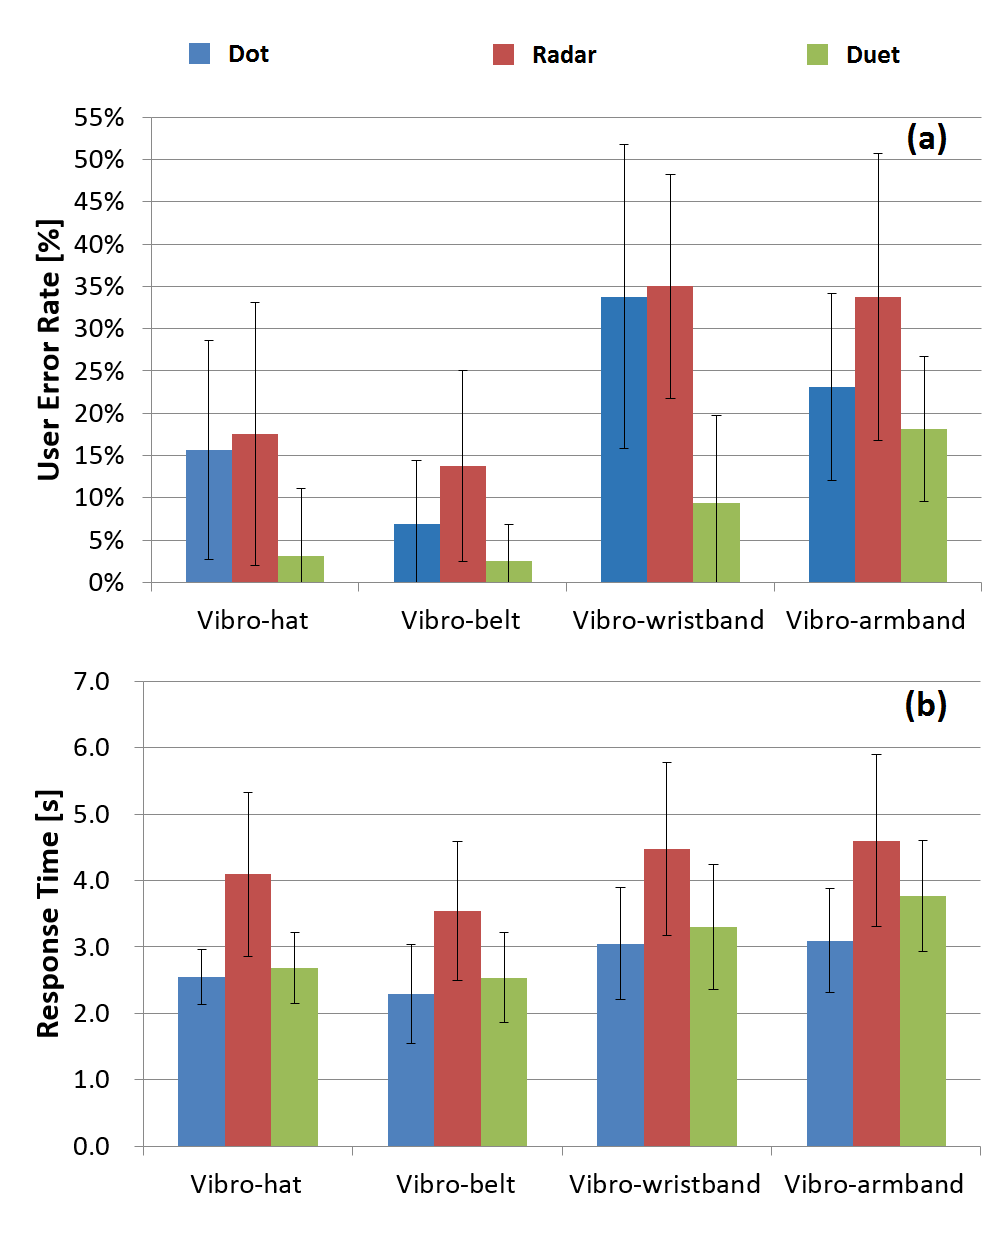
\includegraphics[width=\columnwidth]{stage1_Vibro_ER&RT}
\caption{Mean error rate: Vibro-tactile devices.}
\label{fig:vibro_ER&RT}
\end{figure}

%\begin{figure}[!t]
%\centering
%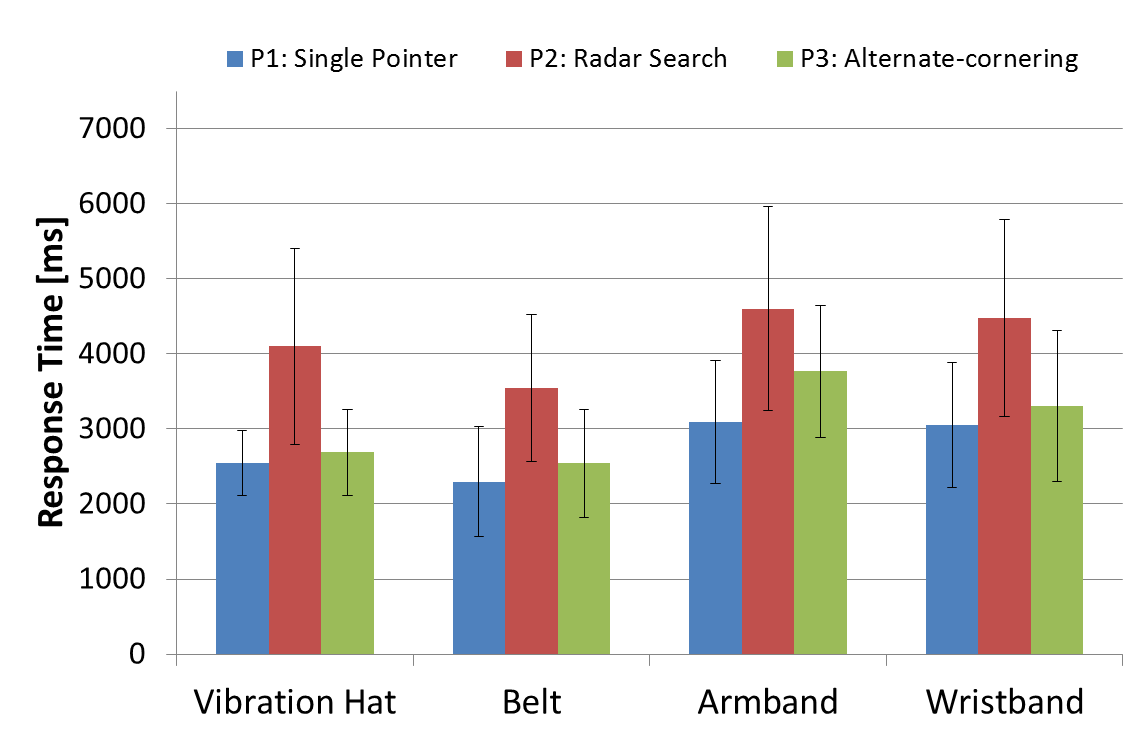
\includegraphics[width=\columnwidth]{Vibro_RT}
%\caption{Mean response time: Vibro-tactile devices.}
%\label{fig:Vibro_RT}
%\end{figure}

\subsection{Experiment 1B Result: Tactile Display}
The results from experiment 1A are summarized in Figure~\ref{fig:vibro_ER&RT} showing detection error rates and response times respectively. The result of which is statistically significant (F(11,108)=9.137,p=0). The first pattern has shortest response time on every device (from 2290 ms to 3090 ms). Almost all users said that it is difficult to distinguish patterns when the density of the vibrators is too high, such as wristband or armband. The second pattern has high marks on both error rate (13.7\% to 35\%) and response time (3540 ms to 4480 ms). On contrary, the third pattern has the lowest error rate with a significant difference (p\textless0.05) on every device but however the response time is nearly equal to first pattern, and the users reports the direction can be clearly distinguished. Among all tactile accessories, armband has the highest error rate of 18.8\% to 33.8\% and response time of 3090 to 4600 ms on all patterns. It is evident in the questionnaire that armband is the least preferred overall.

\subsection{Experiment 1B Conclusion}
During the pilot study, we know that it is confusing for user to distinguish the pattern of vibration if there are more than one vibrator activate at the same time. Since the tactile sense will be disturbed when the vibrators' position are near. Our result show the armband and wristband have high error rate due to the high density of vibrators. The reason for this issue is caused by the design limitation of small surface contact area on the wrists and arms. And we also suspect that it was caused by the long time lapse between each cycle. Overall, the third pattern performed better than the second pattern in terms of the error rate and response time. This difference is statically significant (p\textless0.05). In addition, we found that complex patterns will result in skin numb.

Although the error rate of third pattern for wristband is relatively higher than those in belt and hat, its performance, is however higher than the other two patterns. Since the third display method reduced vibrator density into half by cutting down units of vibrators to four. This is evident that the error rate of the first pattern on both belt and armband is lower than pattern two (p\textless0.05). In addition, its performance is similar to the third pattern on the same devices. However, from the questionnaire, we observed a higher preferences by users on the third pattern due to its clear and easy to comprehend display pattern. In conclusion, we've selected pattern three of all devices to continue the study for the next experiment.

\section{Experiment 2}
\subsection{Experiment Description}
This part of the study was designed to evaluate the usability of our devices and feedbacks selected from the previous experiment for the hearing impaired in particular. We conducted analysis on user's workload for each test by using NASA Task Load Index (TLX), a subjective, multidimensional assessment tool that rates perceived workload based on six aspects: mental demand, physical demand, temporal demand, performance, effort, and frustration. In addition, users’ preferences on each accessories are accessed during a short interview. In the second experiment, all of the proposed devices and remaining display patterns chosen from the previous experiment will be used. In short, there are three goals to reach and discuss in this experiment: 1) investigation of perceptual assistance of sound source direction for people with hearing loss, 2) the comparison of efforts among completing tasks between each devices, and 3) explore user preferences from ratings and feedbacks.

\subsection{Apparatus}

\begin{figure}[!t]
\centering
\includegraphics[width=0.6\columnwidth]{apparatus3}
\caption{Test environment setup for experiment 2: Participants is surrounded by 8 speakers, and a laptop is set in front of the subject.}
\label{fig:speakers}
\end{figure}
Six devices were compared in the experiment: glasses, LED cap, smartwatch, vibration hat, belt, and wristband. The armband was taken out of the list due to its low performance and cause of frustration to the users.

The tests were conducted in a sound environment in order to simulate real life scenario. The subject was seated in the center of a circle (diameter 3 m). Eight loudspeakers were placed on the periphery of the circle with a 45$^\circ$ separation to represent the sound source of eight directions (see Figure~\ref{fig:speakers}). During the test, an Arduino was used to choose which speaker to play the sound. A sequence of car horn in traffic were played by one of the eight speaker to simulate an incoming sound from the according direction. To prevent discomfort to participant caused by speaker noise. All loudspeakers are measured to play at the volume of approximately 65$\sim$70 dB. (The range of 60$\sim$70 dB, or decibels sound pressure level is about as loud as normal conversation in one meter distance. Car horns in average produce 110 dB.) At the meanwhile, tactile or visual device will perform the cue pattern corresponded to the direction of the playing speaker. A laptop was set in front of the participant to display the simulation video.

\begin{figure}[!h]
\centering
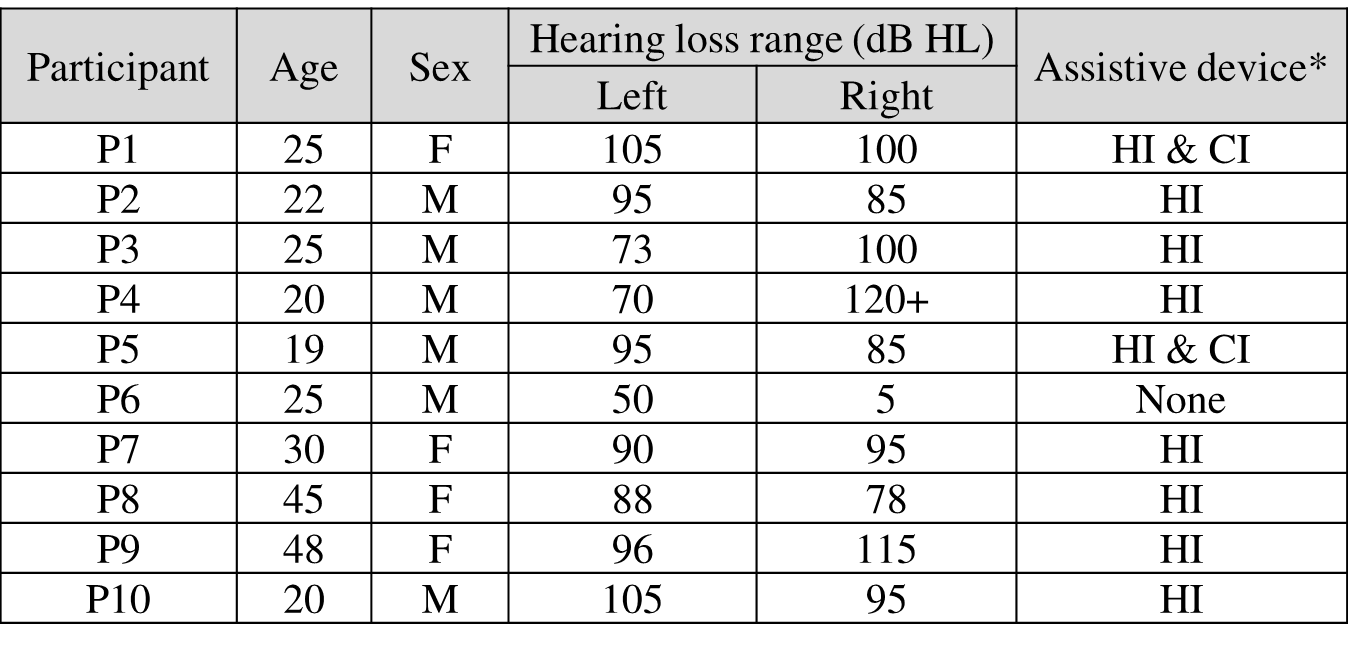
\includegraphics[width=\columnwidth]{participants}
\caption{Mean error rate: Visual devices.}
\label{fig:participants}
\end{figure}

\subsection{Participants}
We recruited 10 hearing impaired participants (4 females, average 29) to take part in the second experiment (Figure \ref{fig:participants}). Subjects are students and school staffs from campus. There are 1 moderately-severe deaf, 5 severely deaf, and 3 profoundly deaf. Nine participants wear hearing aids in daily bases, and two of them have cochlear implants. During the experiment, all participants were asked to configure their hearing instruments to normal settings used in daily life in order to prevent biases.

The severity of a hearing impairment is ranked according to the additional intensity above a nominal threshold that a sound must be before being detected by an individual; it is (measured in decibels of hearing loss, or dB HL). Hearing impairment may be ranked and defined as below \cite{Elzouki2012}:

\begin{itemize}
\item Mild: between 26 and 40 dB HL (adults); between 20 and 40 dB HL (children)
\item Moderate: between 41 and 54 dB HL
\item Moderately severe: between 55 and 70 dB HL
\item Severe: between 71 and 90 dB HL
\item Profound: 91 dB HL or greater
\end{itemize}

\subsection{Procedure}
The procedure in experiment 2 is similar to experiment 1, except that participants were asked to look at the video played on the laptop. The test was to simulate a driving scenario which the subjects was told to be either a car driver, a motorcyclist, or a bicyclist as they wish. Subjects determine the direction till received an indication of a directional signal either from the playing speaker or from the wearable device. The experiment was structured into seven tests. The first test investigates subject's ability of identifying sound direction without the help from our device. Participants in the first test wear only hearing aid and/or cochlear implant. Later on, 6 wearable devices were put on to complete the rest of the tests. The order of devices in each experiment was counter balanced.

As the previous experiment, 16 trials of randomly generated tasks are presented in each test. Participants are given 90 seconds to memorize the cue patterns. When the test begin, participants have 15 seconds to select the accounted direction. We recorded the response time and answers of each trial throughout the experiment. At the end of each test, a TLX questionnaire were filled by participant. And for each device, the comfort level, efficiency and willingness of use were rated respectively. Lastly, after all the tests were finished, a cross-device comparison of the same questions was accessed and put into order from the most favorable to the least.

\subsection{Experiment 2 Result}
After the experiment, we recorded the response time and calculated the mean error rate of each participant with each device. The results are summarized in Figure~\ref{fig:stage2_ER&RT}. The chart shows the results of subject's performance with wearing only hearing devices (HI \& CI) and with the help of our devices. As shown in the chart, when participants are not wearing any of our devices, an average error rate of 64.38\% were presented in the first tests. An analysis of variance showed this difference to be highly significant (F(6,63)=69.632, p=0). The lack of accuracy is significantly higher than when the devices are worn (p\textless.00001). Among all proposed devices, the wristband has the highest mean error rate at 10.63\%. On the other hand, smartwatch and vibration belt have the lowest average in error rate with 0.63\%. Nonetheless, except for wristband, vibro-tactile devices has relatively lower or equal error rates to visual display devices.

In term of time consumption, vibration hat has the shortest response time in average (2538 ms) among all the vibro-tactile devices. Whereas the wristband had the longest response time at 3740 ms. Smartwatch on the other hand, has the shortest mean response time at 2149 ms, with a close match to the glasses at 2253 ms. The LED cap in this case consumed a bit longer time with 2716 ms. From the result of the NASA-TLX ratings, vibration wristband had the highest mark on all subscale in NASA-TLX, and smartwatch was the second highest in physical demand (see Figure~\ref{fig:nasa_tlx}). 

To fit the condition in daily life, when smartwatch is worn, we instructed the participants to rest their arms before each notification is presented to prevent them from looking at the screen constantly. For this reason, more physical activity is required to obtain information. This argument is confirmed by the NASA-TLX scale, which shows the smartwatch received higher score on physical demand than any other devices. However, this result does not correspond to the mean response time recorded from the tests (2149 ms, the lowest among all). Furthermore, the result stated that the average response time of vibration devices (3009 ms) are longer than those of visual devices (2373 ms) except for the LED cap.

\subsubsection{Questionnaire}


\begin{figure}[!t]
\centering
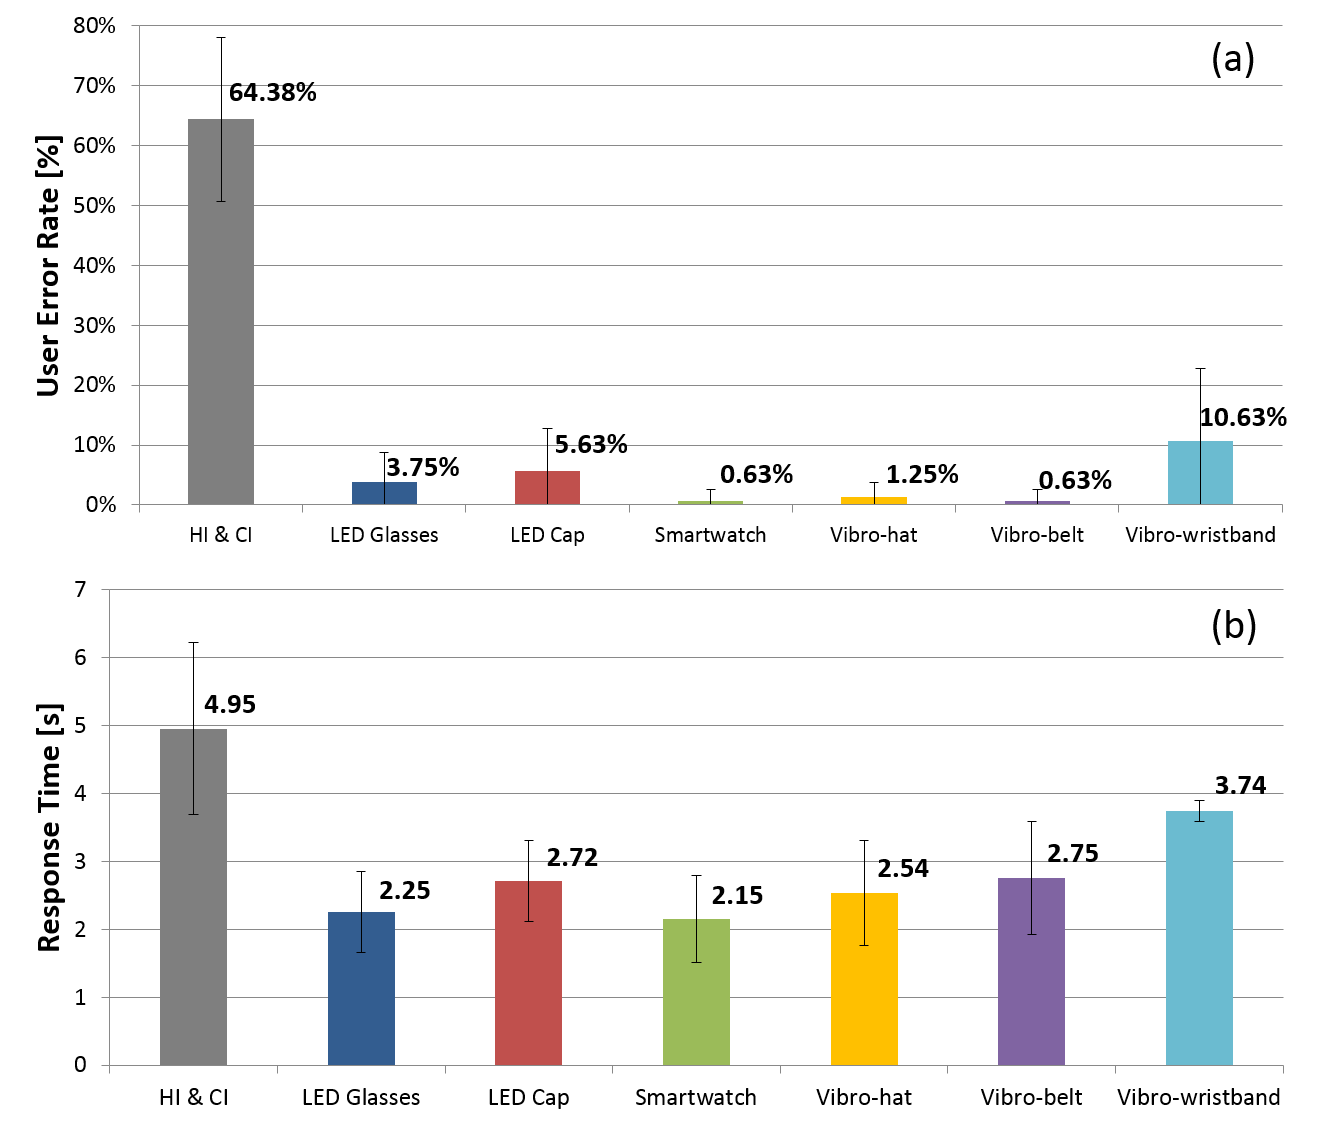
\includegraphics[width=\columnwidth]{stage2_ER&RT}
\caption{Mean error rate: All devices.}
\label{fig:stage2_ER&RT}
\end{figure}

\begin{figure}[!t]
\centering
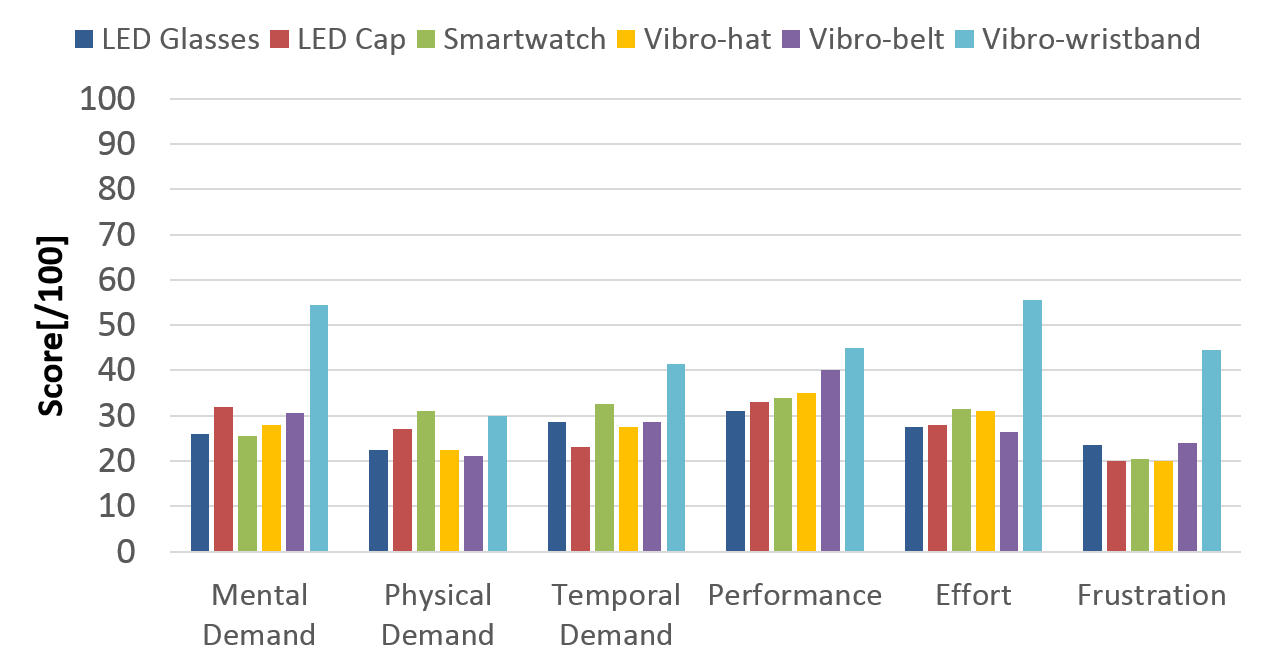
\includegraphics[width=\columnwidth]{stage2_TLX}
\caption{Mean score of NASA Task Load Index for each device.}
\label{fig:nasa_tlx}
\end{figure}

\begin{figure}[!t]
\centering
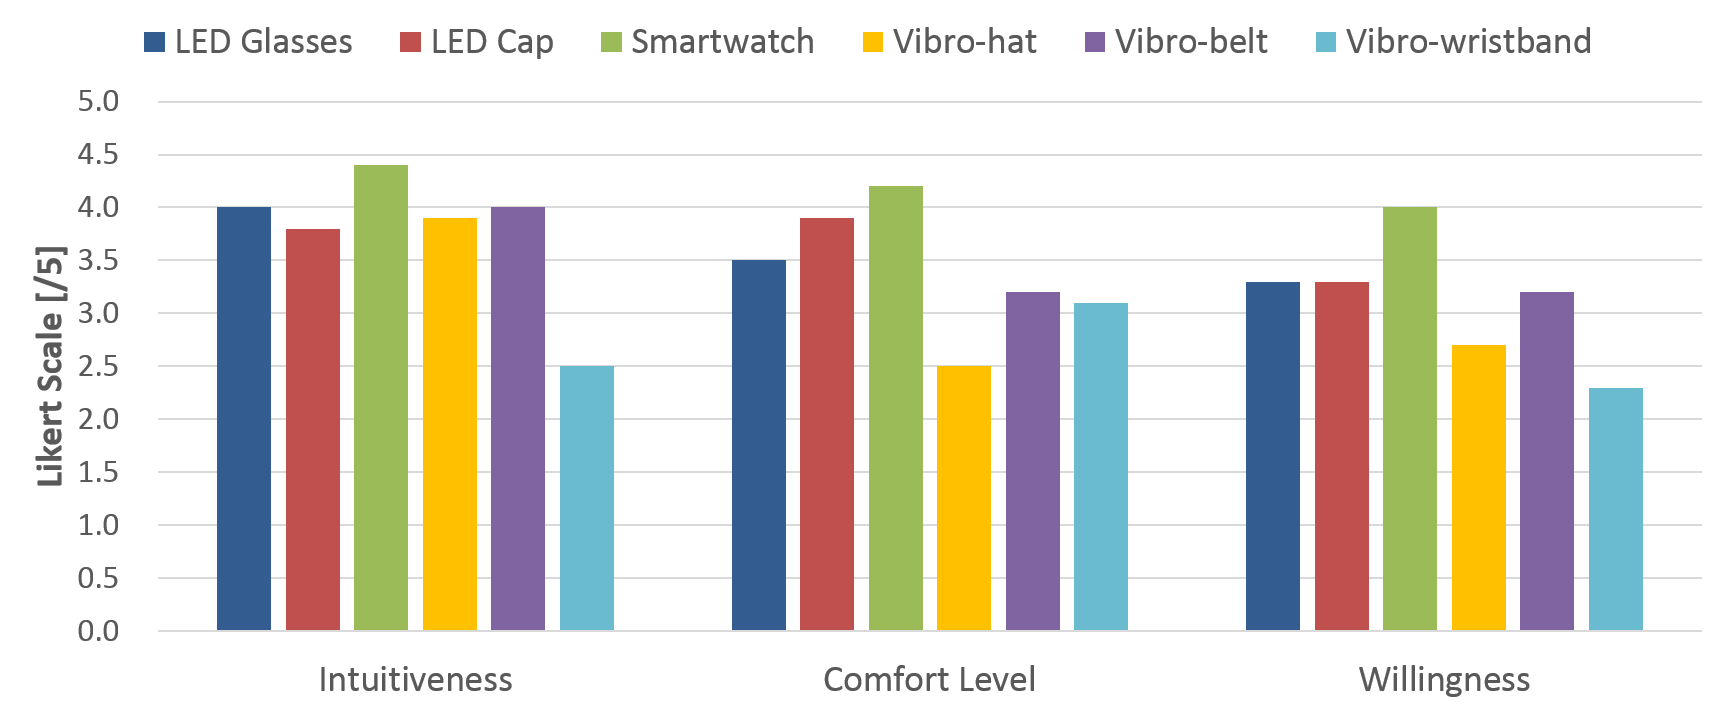
\includegraphics[width=\columnwidth]{stage2_Likert}
\caption{User's preference on a five-point Likert scale.}
\label{fig:likert_scale}
\end{figure}

In addition to the workload index estimated by NASA-TLX. The participants assessed 3 statements at the end of each 6 devices about the intuitiveness of recognizing sound direction, the comfort level of the display method, and the willingness to use our devices. %These ratings are shown in Figure~\ref{fig:Likert_Intuitive} to ~\ref{fig:Likert_Wanted}.
A continuous rating scale from 1 (\textquoteleft strongly disagree\textquoteright) to 5 (\textquoteleft strongly agree\textquoteright) has been used and the participants had to give a score depending on the agreement level of the statement. At the end of the questionnaire, the participants had the opportunity to answer several open questions in regards to improvements and general comments.

The visual devices (smartwatch, glasses, and LED cap) were evaluated more efficient than the vibration devices (vibration hat, vibration belt, and vibration wristband). However, three participants mentioned that they spent more times to memorize the patterns of LED cap than others. Smartwatch was rated as the most intuitive device. In contrast, vibration wristband was rated the least. Almost all of the participants reported that it is difficult to identify the vibration signal from the wristband since vibration units are too close to each other. \textit{\textquotedblleft It feels like the whole wrist is shaking,\textquotedblright} stated by two of the participants. Few participants mentioned that recognizing diagonal directions in vibration belt and hat are time-consuming. Since two vibrators are activated alternatively, it requires user to make sure two vibrators are presented in order to determine directions. Two of the participants said that it is hard to distinguish the lights on the lower corners of glasses from the bottom; one due to the reason of \textit{\textquotedblleft too close to each other\textquotedblright}, and other might be caused by nearsightedness.

In comparison of comfort level, smartwatch was rated the most comfortable whereas vibration hat was rated as the least. Besides, three participants mentioned that noise and disturbance was caused by vibration to the hearing aids while using vibration hat. Some said that they felt uncomfortable by the sudden shock of vibration. In addition, few of participants stated that the lights on the LED glasses are too bright.

Most participants showed a high willingness of using smartwatch. On the contrary, vibration hat received the lowest score in willingness. Furthermore, we noticed that younger participants find LED cap more helpful than the elder ones. They assume the reason might be that younger users have better performance in remembering the patterns than the elders.

\subsection{Experiment 2 Conclusion}
After experiment 2 was conducted, it is clear that our devices has significantly improved users perception on sound source direction detection. Even though most tactile devices have relatively low error rates than visual devices, user feedbacks from the questionnaire shows a higher intuitive level of visual devices than that of tactile devices. This explained why visual devices had shorter response time than most tactile devices. Moreover, from the questionnaire, it seems that the factor of which the willingness of using a device is firstly based on the level of comfort instead of its efficiency. It also showed that the vibration hat, LED glasses, and smartwatch can cause distraction to user's attention. Although more than half of the participants complained about vibration hat, its error rate is surprisingly low. Therefore, without effecting the performance, we believe the discomfort of the vibration can be improved through adjustment of intensity and a better hardware design.

\section{Conclusion and Discussion}
We have proposed several design of wearable devices with different display methods. The study focused on supporting auditory perception for people with hearing loss to recognize directions of environmental sound. Experiments were conducted with both hearing and deaf individuals to evaluate various type of visual and vibratory-coded devices. Our results showed a significant improvement in deaf users' acoustic awareness to sound source direction when our devices are implemented. Furthermore, we discussed the usability and performances on each of the device and proposed encoding schemes based on several aspects, which are level of comfort in regards of the display methods, intuitiveness on recognizing cue patterns, and willingness to use such devices.

Our findings have a number of implications for the use of wearable visual and vibro-tactile interfaces. We discovered human's vision and tactile sensory capability is limited in processing complex information, especially when it is encoded. Using imagery information or simple coded pattern to represent direction is more efficient. Using of appropriate lighting intensity to avoid blinding or exhaustion to human eyes is critical. On the other hand, human's sensibility to vibro-tactile stimuli is also varied on different parts of the body location. For instance, head and waist are highly sensitive to tactual stimulation. But due to the reason that these body parts have larger surface contact area than wrist or arms. Therefore, even though users felt uncomfortable or ticklish when tactual sensation are applied on these body parts, they however performed a better result in directional interpretation. Furthermore, it is important to avoid a design with high density vibrator display.

As part of the result, smartwatch seems to have a good performance and high preferences overall. Since users tend to prefer using direct imagery to present directional information. Whether or not it would be useful if they are presented directly in sight is an interesting topic to discover. A possible implementation is using heads-up display to perform imagery information directly to users eyes. Without the need of extra physical activity such as moving the head or raising the arm, it may introduce less interference to user's visual attention to the environment, and may as well improve reaction time.

Another question we are interested to find out is how to express different types of characteristics of sound simultaneously through visual or tactile expression. For example, an interface that can display not only directional information of sound but intensity, distance, level of emergencies and other factors that can help people with hearing loss improve perception and awareness of the environmental sound.

\balance

% If you want to use smaller typesetting for the reference list,
% uncomment the following line:
%\small
\bibliographystyle{acm-sigchi}
\bibliography{visso}
\end{document}
